% Evaluation %
\chapter{Evaluation}
\label{chapter5}
In Chapter~\ref{chapter3} we have shown which basic concepts have been used and in Chapter~\ref{chapter4} it was shown how this concepts can be applied to develop the \TOOL. In order to demonstrate that the goals regarding the included functionality have been achieved and also to show that the use of the tool is time efficient, a detailed analysis will be carried out. The first step is to check if the \TOOL provides the desired functionality and whether it can be applied to different applications. For this purpose, four programs of different complexity levels will be analyzed and transformed with the \TOOL. The programs created can then be analyzed. The performance of the \TOOL is to be tested by frequently running four applications in different environments. This allows the time of a program without performance counters to be compared with a program to which they have been added.

\section{Functional Analysis}
This section aims to demonstrate the effectiveness of the approach by showing the measurement results available through the application of the \TOOL. To show this, three programs of varying complexity are selected. Each application is analyzed with the \TOOL until a code region with a high resource consumption is found. The results of the measurements are presented and discussed for each hierarchy. In Section~\ref{overheadAnalysis}, the overhead generated by inserting measurement code into the benchmark programs is discussed in detail. 

\subsection{Varying Loop Runtimes}
As a first example, let us analyze the code framework shown in the introduction. For this purpose, the basic structure is extended with several instructions, so that the code looks similar to the code shown in Listing~\ref{lst:e:perf_forloops}. It can be seen that three \lstinline{for}-loops are executed in the main function, each loop performing a simple task a thousand times. The first loop writes a string to the command line, the second performs a multiplication of two numbers, and the last adds items to a shopping list and then sorts them. 

\begin{lstlisting}[float, language=C++, caption=\CPP Code Showing the \VARYINGLOOP Application., label=lst:e:perf_forloops]
#include <iostream>
#include <vector>

int main(void) {
    for ( int i = 1; i <= 1000; i++ ) {
        std::cout << "Hello World";
    }
    for ( int i = 1; i <= 1000; i++ ) {
        int numberA = 892346;
        int numberB = 384378;
        int numberC = numberA * numberB;
    }
    for ( int i = 1; i <= 1000; i++ ) {
        std::vector<std::string> shoppingList;
        shoppingList.push_back("Milk");
        shoppingList.push_back("Eggs");
        shoppingList.push_back("Meat");
        shoppingList.push_back("Water");
        shoppingList.push_back("Sugar");
        shoppingList.push_back("Flour");
        shoppingList.push_back("Salt");
        std::sort( shoppingList.begin( ), shoppingList.end( ));
    }
    return 0;
}
\end{lstlisting} 

The first step is to use the \TOOL to add measurement code to the source application. This requires executing the instructions shown in Listing~\ref{lst:e:terminal_instructions}. Initially, the \TOOL is called with the source code as input. The \TOOL analyzes the code, adds performance counters around the \roismall, and returns a modified \CPP application. The program created can then be compiled into an executable application. The last step is to execute the created software. Since these steps work the same for all programs, we will not specify them separately.

\begin{lstlisting}[float, language=C++, caption={Instructions for Transformation, Compilation and Execution.}, label=lst:e:terminal_instructions]
/* source-to-source transformation with the roiprofiler */
roiprofiler VaryingLoopRunTimes.cpp

/* compilation of the generated code */
clang++ VaryingLoopRunTimes.cpp -o application

/* execution of the binary file */
./application
\end{lstlisting} 

The transformed program writes the results of the tasks and the statistics of the running times, which can be seen in Table~\ref{tab:e:forloops_output}, to the command line. The data provided shows at a glance that the last loop, which creates and sorts shopping lists, consumes the most amount of time. Furthermore, it can be seen that the first loop requires the second most resources and that the runtime of the second loop is almost negligible. If the user wants to improve performance based on this data, priority should be given to the level below the third loop.

\begin{table}
  \centering
  \caption{Runtime Evaluation for the \VARYINGLOOP Application.}
  \begin{tabular}{rrrrrr}
    \toprule
    Identifier & ClassType & Runtime                      & Scope \%              & Total \%              & Calls \\
    \midrule
    2192956    & ForStmt   & \SI{402.291}{\micro\second}  & \SI{4.62}{\percent}   & \SI{4.62}{\percent}   & 1     \\
    2193096    & ForStmt   & \SI{2.671}{\micro\second}    & \SI{0.03}{\percent}   & \SI{0.03}{\percent}   & 1     \\
    2225085    & ForStmt   & \SI{8303.364}{\micro\second} & \SI{95.34}{\percent}  & \SI{95.34}{\percent}  & 1     \\
    Overhead   &           & \SI{0.626}{\micro\second}    & < \SI{0.01}{\percent} & < \SI{0.01}{\percent} & 12    \\
    \midrule
    Runtime    &           & \SI{8709.478}{\micro\second} &                       &                       &       \\
    \bottomrule
  \end{tabular}
  \label{tab:e:forloops_output}
\end{table}

\subsection{Fibonacci Sequence}
\label{sectionFibonacciCode}
As a next example we want to analyze the \FIBONACCI program that calculates the first thousand numbers of the Fibonacci sequence. The code of the application is shown in Listing~\ref{lst:e:perf_fibonacci}. We will follow the same process as in transforming the previous program to obtain the statistics shown in Table~\ref{tab:e:fibonaccioutput1}.

\begin{lstlisting}[float, language=C++, caption=\CPP Code Showing the \FIBONACCI Application., label=lst:e:perf_fibonacci]
#include <iostream>

int main(void) {
    double n, t1 = 0, t2 = 1, nextTerm = 0;
    n = 1000;

    std::cout << "Fibonacci Series: ";

    for (int i = 1; i <= n; ++i) {
        if(i == 1) {
            std::cout << t1;
            std::cout << ", ";
        }
        else if(i == 2) {
            std::cout << t2;
            std::cout << ", ";
        }
        nextTerm = t1 + t2;
        t1 = t2;
        t2 = nextTerm;

        std::cout << nextTerm << ", ";
    }

    return 0;
}
\end{lstlisting} 

\begin{table}
  \centering
    \caption{Runtime Evaluation for the \FIBONACCI Application.}
  \begin{tabular}{rrrrrr}
    \toprule
    Identifier & ClassType          & Runtime                       & Scope \%             & Total \%             & Calls \\
    \midrule
    i000002    & CustomCompoundStmt &  \SI{23.649}{\micro\second}   & \SI{2.29}{\percent}  & \SI{2.29}{\percent}  & 1     \\
    2086033    & ForStmt            &  \SI{1007.385}{\micro\second} & \SI{97.70}{\percent} & \SI{97.66}{\percent} & 1     \\
    Overhead   &                    &  \SI{0.108}{\micro\second}    & \SI{0.01}{\percent}  & \SI{0.01}{\percent}  & 6     \\
    \midrule
    Runtime    &                    &  \SI{1031.509}{\micro\second} &                      &                      &       \\
    \bottomrule
  \end{tabular}
  \label{tab:e:fibonaccioutput1}
\end{table}

It can be seen that the \lstinline{for}-loop consumes almost all of the runtime, so in this case it is not clear which region is to be revised. Therefore, the \TOOL must be called again with the parameter \lstinline{--stmt 2086033}, which results in the statistics shown in Table~\ref{tab:e:fibonaccioutput2}. In this output, the higher runtime is noticeable, which arises because a calculation of the runtime must be carried out for each loop cycle. In total, the execution of the program now took \SI{500}{\micro\second} longer, whereby it can be seen that about half of the overhead occurred could be recognized by the \TOOL and shifted to a separate area. This occurs because a \DECL is made first and only then the current time is written to memory. Thus, the overhead caused by measuring the start time of an instruction can be eliminated, but not the time required to declare the end time. This occurrence will be discussed in more detail in the overhead analysis in Section~\ref{overheadAnalysis}. Looking at the table again, it can be seen that the \lstinline{CustomCompoundStmt} takes up about seventy-five percent of the runtime and the instructions inside it are executed a thousand times. The reason for the high runtime consumption is that the calculations in both the \lstinline{if}- and the \lstinline{else-if}-branch are only executed once, while all other instructions are executed every time. Furthermore, it is noticeable that a scope runtime is now specified that contains the duration of all instructions below the user-specified \emph{region of interest}. In this application, it was also possible to find a region that has a high resource consumption. 

\begin{table}
  \centering
    \caption{Runtime Evaluation for the \lstinline{ForStmt} of the \FIBONACCI Application.}
  \begin{tabular}{rrrrrr}
    \toprule
    Identifier & ClassType          & Runtime                      & Scope \%             & Total \%             & Calls \\
    \midrule
    2085332    & IfStmt             & \SI{140.928}{\micro\second}  & \SI{9.27}{\percent}  & \SI{9.13}{\percent}  & 1000  \\
    i000004    & CustomCompoundStmt & \SI{1153.832}{\micro\second} & \SI{75.91}{\percent} & \SI{74.71}{\percent} & 1000  \\
    Overhead   &                    & \SI{225.283}{\micro\second}  & \SI{14.82}{\percent} & \SI{14.59}{\percent} & 4004  \\
    \midrule
    Scope      &                    & \SI{1520.043}{\micro\second} &                      &                              \\
    Runtime    &                    & \SI{1544.359}{\micro\second} &                      &                              \\
    \bottomrule
  \end{tabular}
  \label{tab:e:fibonaccioutput2}
\end{table}

\subsection{Password Generator}
\label{sectionPasswordCode}
Next, a slightly more resource-intensive application will be tested, whereby the aim will also be to find the instruction that consumes the longest amount of time. For this purpose, the \PASSWORDGEN program shown in Listing~\ref{lst:e:perf_passwords} will be analyzed in more detail. The program generates one million passwords, each containing three sections of six characters. After all passwords have been generated, the list is sorted and duplicates are eliminated. The sorted passwords are finally displayed to the user on the command line. In this example, it is particularly interesting to see if the generation of the passwords or the actions on the data structure require more time.

\begin{lstlisting}[float, language=C++, caption=\CPP Code Showing the \PASSWORDGEN Application., label=lst:e:perf_passwords]
#include <string>
#include <vector>
#include <iostream>

int main(void) {
    std::vector <std::string> passwordStorage;
    std::string password;
    char current;

    for (int passwordCount = 0; passwordCount < 1000000; passwordCount++) {
        for (int sectionCount = 0; sectionCount < 3; sectionCount++) {
            for (int sectionLength = 0; sectionLength < 6; sectionLength++) {
                char lowerCase = rand() % 26 + 'a';
                char upperCase = rand() % 26 + 'A';
                char number = rand() % 10 + '0';

                char randomChoice = (rand() % 100 + 1);
                if (randomChoice <= 40) {
                    current = lowerCase;
                } else if (randomChoice <= 80) {
                    current = upperCase;
                } else {
                    current = number;
                }
                password += current;
            }
            password += '-';
        }
        password.pop_back();
        passwordStorage.push_back(password);
        password.clear();
    }

    std::sort(passwordStorage.begin(), passwordStorage.end());
    passwordStorage.erase(std::unique(passwordStorage.begin(),
                                            passwordStorage.end()),
                          passwordStorage.end());

    for (std::string currentPassword: passwordStorage) {
        std::cout << currentPassword << '\n';
    }

    return 0;
}
\end{lstlisting} 

First of all, an overview of the running times of the first level should be generated, which can be seen in Table~\ref{tab:e:passwordoutput1}. In these statistics, the different runtimes of the various parts of the application can be seen very clearly. It is noticeable that the operations performed on the list require about five times the amount of time it takes to create one thousand passwords. 

\begin{table}
  \centering
  \caption{Runtime Evaluation for the \PASSWORDGEN Application.}
  \begin{tabular}{rrrrrr}
    \toprule
    Identifier & ClassType          & Runtime                      & Scope \%             & Total \%              & Calls \\
    \midrule
    i000002    & CustomCompoundStmt & < \SI{0.001}{\milli\second}  & \SI{9.27}{\percent}  & < \SI{0.01}{\percent} & 1     \\
    2219672    & ForStmt            & \SI{988.027}{\milli\second}  & \SI{75.91}{\percent} & \SI{16.07}{\percent}  & 1     \\
    i000005    & CustomCompoundStmt & \SI{5161.804}{\milli\second} & \SI{9.27}{\percent}  & \SI{83.93}{\percent}  & 1     \\
    Overhead   &                    & < \SI{0.001}{\milli\second}  & \SI{14.82}{\percent} & < \SI{0.01}{\percent} & 8     \\
    \midrule
    Runtime    &                    & \SI{6149.833}{\milli\second} &                      &                       &       \\
    \bottomrule
  \end{tabular}
  \label{tab:e:passwordoutput1}
\end{table}

Table~\ref{tab:e:passwordoutput2} shows the statistics of the analysis of the innermost for loop. It can be seen that the added performance counters consume more runtime than the actual instructions. This is due to the fact that six times per loop pass are measured, resulting in a total of 108 million \MEASUREVALUES recorded.

\begin{table}
  \centering
  \caption{Runtime Evaluation for the \lstinline{ForStmt} of the \PASSWORDGEN Application.}
  \begin{tabular}{rrrrrr}
    \toprule
    Identifier & ClassType     & Runtime                       & Scope \%             & Total \%             & Calls    \\
    \midrule
    i000002    & CCompoundStmt & \SI{1857.092}{\milli\second}  & \SI{20.11}{\percent} & \SI{12.55}{\percent} & 1,8E+07  \\
    2219672    & IfStmt        & \SI{1556.085}{\milli\second}  & \SI{16.85}{\percent} & \SI{10.51}{\percent} & 1,8E+07  \\
    i000005    & CCompoundStmt & \SI{1529.157}{\milli\second}  & \SI{16.56}{\percent} & \SI{10.33}{\percent} & 1,8E+07  \\
    Overhead   &               & \SI{4292.683}{\milli\second}  & \SI{46.48}{\percent} & \SI{29.00}{\percent} & 1,08E+08 \\
    \midrule
    Scope      &               & \SI{9235.017}{\milli\second}  &                      &                      &          \\
    Runtime    &               & \SI{14800.639}{\milli\second} &                      &                      &          \\
    \bottomrule
  \end{tabular}
  \label{tab:e:passwordoutput2}
\end{table}

\subsection{Prime Benchmark}
\label{sectionPrimeCode}
Finally, we want to examine an application that calculates as many prime numbers as possible within a period of \SI{5}{\second}. For this purpose, we will use the code that is freely available under the GitHub repository ``PlummersSoftwareLLC/Primes''~\cite{PrimeBenchmark}. The calculation of prime numbers is often used to benchmark the performance of a processor. The \TOOL is used to find out which part of the software takes the longest time. 

\begin{lstlisting}[float, language=C++, caption=Output of the \PRIME Application., label=lst:e:primeoutput_terminal]
Passes: 1033, Time: 5.000021;1;algorithm=base,faithful=yes,bits=1
\end{lstlisting}

\begin{table}
  \centering
  \caption{Runtime Evaluation for the \PRIME Application.}
  \begin{tabular}{rrrrrr}
    \toprule
    Identifier & ClassType          & Runtime                      &  Scope \%             &  Total \%             & Calls \\
    \midrule
    i000002    & CustomCompoundStmt & \SI{4.063}{\milli\second}    & \SI{0.08}{\percent}   & \SI{0.08}{\percent}   & 1033  \\
    2418305    & CXXMemberCallExpr  & \SI{499.446}{\milli\second}  & \SI{99.59}{\percent}  & \SI{99.59}{\percent}  & 1033  \\
    i000004    & CustomCompoundStmt & \SI{0.126}{\milli\second}    & < \SI{0.01}{\percent} & < \SI{0.01}{\percent} & 1033  \\
    2420840    & IfStmt             & < \SI{0.001}{\milli\second}  & < \SI{0.01}{\percent} & < \SI{0.01}{\percent} & 1033  \\
    Overhead   &                    & \SI{21.125}{\milli\second}   & \SI{0.42}{\percent}   & \SI{0.42}{\percent}   & 8266  \\
    \midrule
    Scope      &                    & \SI{5014.148}{\milli\second} &                       &                       &       \\
    Runtime    &                    & \SI{5014.148}{\milli\second} &                       &                       &       \\
    \bottomrule
  \end{tabular}
  \label{tab:e:primeoutput1}
\end{table}

The result generated by the \PRIME application can be seen in Listing~\ref{lst:e:primeoutput_terminal}. It can be seen that 1033 prime numbers were calculated in this run and that the runtime was approximately \SI{5}{\second}. The generated runtime statistic of the \TOOL can be seen in Table~\ref{tab:e:primeoutput1}. It is clearly visible that the output of the data takes only a fraction of the calculations. 

The next step is to find out which part of the calculation is the most demanding on resources. Therefore, the \TOOL is executed until it reaches the content of the function \lstinline{setFlagsFalse(size_t n, size_t skip)}. The results generated by the \PRIME application are shown in Listing~\ref{lst:e:primeoutput2_terminal}. This time 1020 prime numbers could be calculated in a time span of \SI{5}{\second}, thirteen less than in the last run. The output generated by the \TOOL is shown in Table~\ref{tab:e:primeoutput2}. Compared to the last run, not only 8266 but 685223 time values were calculated, which almost doubled the time used by the counters. In the statistics added by the \TOOL it can be seen that the content of the \lstinline{while}-loop run takes \SI{98.87}{\percent} of the total runtime, and thus the most resource intensive part of the application could be found. However, since there are only \LEASTAS in the \lstinline{while}-loop and these are combined into a \lstinline{CustomCompoundStmt}, there would be no added value for further analysis. Furthermore, at the next stage, the point is reached where more counters are inserted than instructions that are to be measured, causing performance to drop drastically. We will discuss this behaviour in more detail in the overhead analysis of the \PRIME program. 

\begin{lstlisting}[float, language=C++, caption={[Output for the \lstinline{CXXMCall} of the \PRIME Application.]Output for the \lstinline{CXXMemberCallExpr} of the \PRIME Application.}, label=lst:e:primeoutput2_terminal]
Passes: 1020, Time: 5.004809;1;algorithm=base,faithful=yes,bits=1
\end{lstlisting}

\begin{table}
  \centering
  \caption[Runtime Evaluation for the \lstinline{CXXMCall} of the \PRIME Application.]{Runtime Evaluation for the \lstinline{CXXMemberCallExpr} of the \PRIME Application.}
  \begin{tabular}{rrrrrr}
    \toprule
    Identifier & ClassType          & Runtime                      &  Scope \%            &  Total \%            & Calls\\
    \midrule
    i000002    & CustomCompoundStmt & \SI{13.682}{\milli\second}   & \SI{0.27}{\percent}  & \SI{0.27}{\percent}  & 171360 \\
    2420840    & WhileStmt          & \SI{4922.025}{\milli\second} & \SI{98.87}{\percent} & \SI{98.87}{\percent} & 171360 \\
    Overhead   &                    & \SI{42.717}{\milli\second}   & \SI{0.86}{\percent}  & \SI{0.86}{\percent}  & 685442 \\
    \midrule
    Scope      &                    & \SI{4978.425}{\milli\second} &                      &                      &       \\
    Runtime    &                    & \SI{5018.688}{\milli\second} &                      &                      &       \\
    \bottomrule
  \end{tabular}
  \label{tab:e:primeoutput2}
\end{table}

\section{Overhead Analysis}
\label{overheadAnalysis}
In order to determine how many additional resources are consumed by the inserted measurement code, a comprehensive analysis of the runtimes must be carried out. To achieve this, we will run the already known programs \VARYINGLOOP~\ref{lst:e:perf_forloops}, \FIBONACCI~\ref{lst:e:perf_fibonacci}, \PASSWORDGEN~\ref{lst:e:perf_passwords}, and \PRIME~\cite{PrimeBenchmark} in different environments and compare the runtimes. Furthermore, the \PASSWORDGEN program is to be adapted in such a way that this time a number of the passwords to be generated is randomly selected. We will call this application the \VARPASSWORDGEN. Thus, a more precise analysis of the time added by the measurements is possible, since a different number of measured values is recorded in each run. 
\subsection{Method}
All mentioned programs are compiled once without the added performance counter and once after they have been added by the \TOOL. The total runtime of both variants is measured using the \emph{gnu-time} library~\cite{Gtime}. By measuring the total runtime of the processes, it is possible to determine how much more time is required by all the changes made by the \TOOL. The data obtained from this measurement is primarily used to highlight the performance of the calculations and the output. In a second step, the times are measured directly in the \CPP applications using the \CHRONO library. This means that only the pure running times of the instructions can be compared. For this purpose, one timestamp is saved when entering the main function and another one before the definition of the \lstinline{print()} function. This eliminates the overhead that occurs when creating the process as well as the resource consumption of the \lstinline{print()} function. This is especially important because the calculations and the output of the information add more time to the total runtime, but have no influence on the data needed for the profiling evaluation. The information obtained by measuring time with the \CHRONO library gives insight into the overhead caused by the added performance counters themselves. Each program is run a thousand times so that any outliers can be eliminated and an accurate analysis can be made. 

During the analysis we will use the term \MEASUREVALUE when we talk about one measured time, which corresponds to exactly one added counter. A \MEASUREPAIR consists of two \MEASUREVALUES, one recorded before the code block and one recorded after a code block. Further we will talk about the time needed to measure one whole code block. Measuring one code block may require more than one \MEASUREPAIR, since code blocks in loops or recursive functions are measured more than once and the time of each iteration is accumulated. We will call this time the \TOTALCODEBLOCK. 

The programs and scripts used for the analysis are freely available under the GitHub repository ``maxhagn/ROIProfilerCPP''~\cite{ROIPROFILER}, allowing all test steps to be reproduced.

\subsection{Hardware}
In order to test the performance of the \TOOL on hardware of different levels of power, the evaluation is carried out on three systems. First, on a MacBook~Pro Early 2015 with 8~GB 1867~MHz DDR3 memory and a 3.1~GHz dual-core Intel~Core~i7 processor running macOS Monterey version~12.1. The second environment utilizes an 3,8~GHz AMD~Ryzen~9~3900X dodeca-core processor with 96~GB 3200~MHz~DDR4 memory, running ZorinOS~16 based on the Linux Kernel version~5.13.0. The last test device is a iMac~2021 with 8~GB 4266~MHz LPDDR-DDR4X memory and an 3,2~GHz Silicon~M1 octa-core processor, running macOS Monterey version~12.1.

\begin{figure}[t]
  \centering
    \caption[Runtime Comparison for the \VARYINGLOOP Application.]{Runtime Comparison for the \VARYINGLOOP Application. The diagram shows the runtime of each run.  The version of the program without added counters is compared to the version with eight counters added. The trend lines indicate the average runtime. The test was performed on a \AMD.} 
  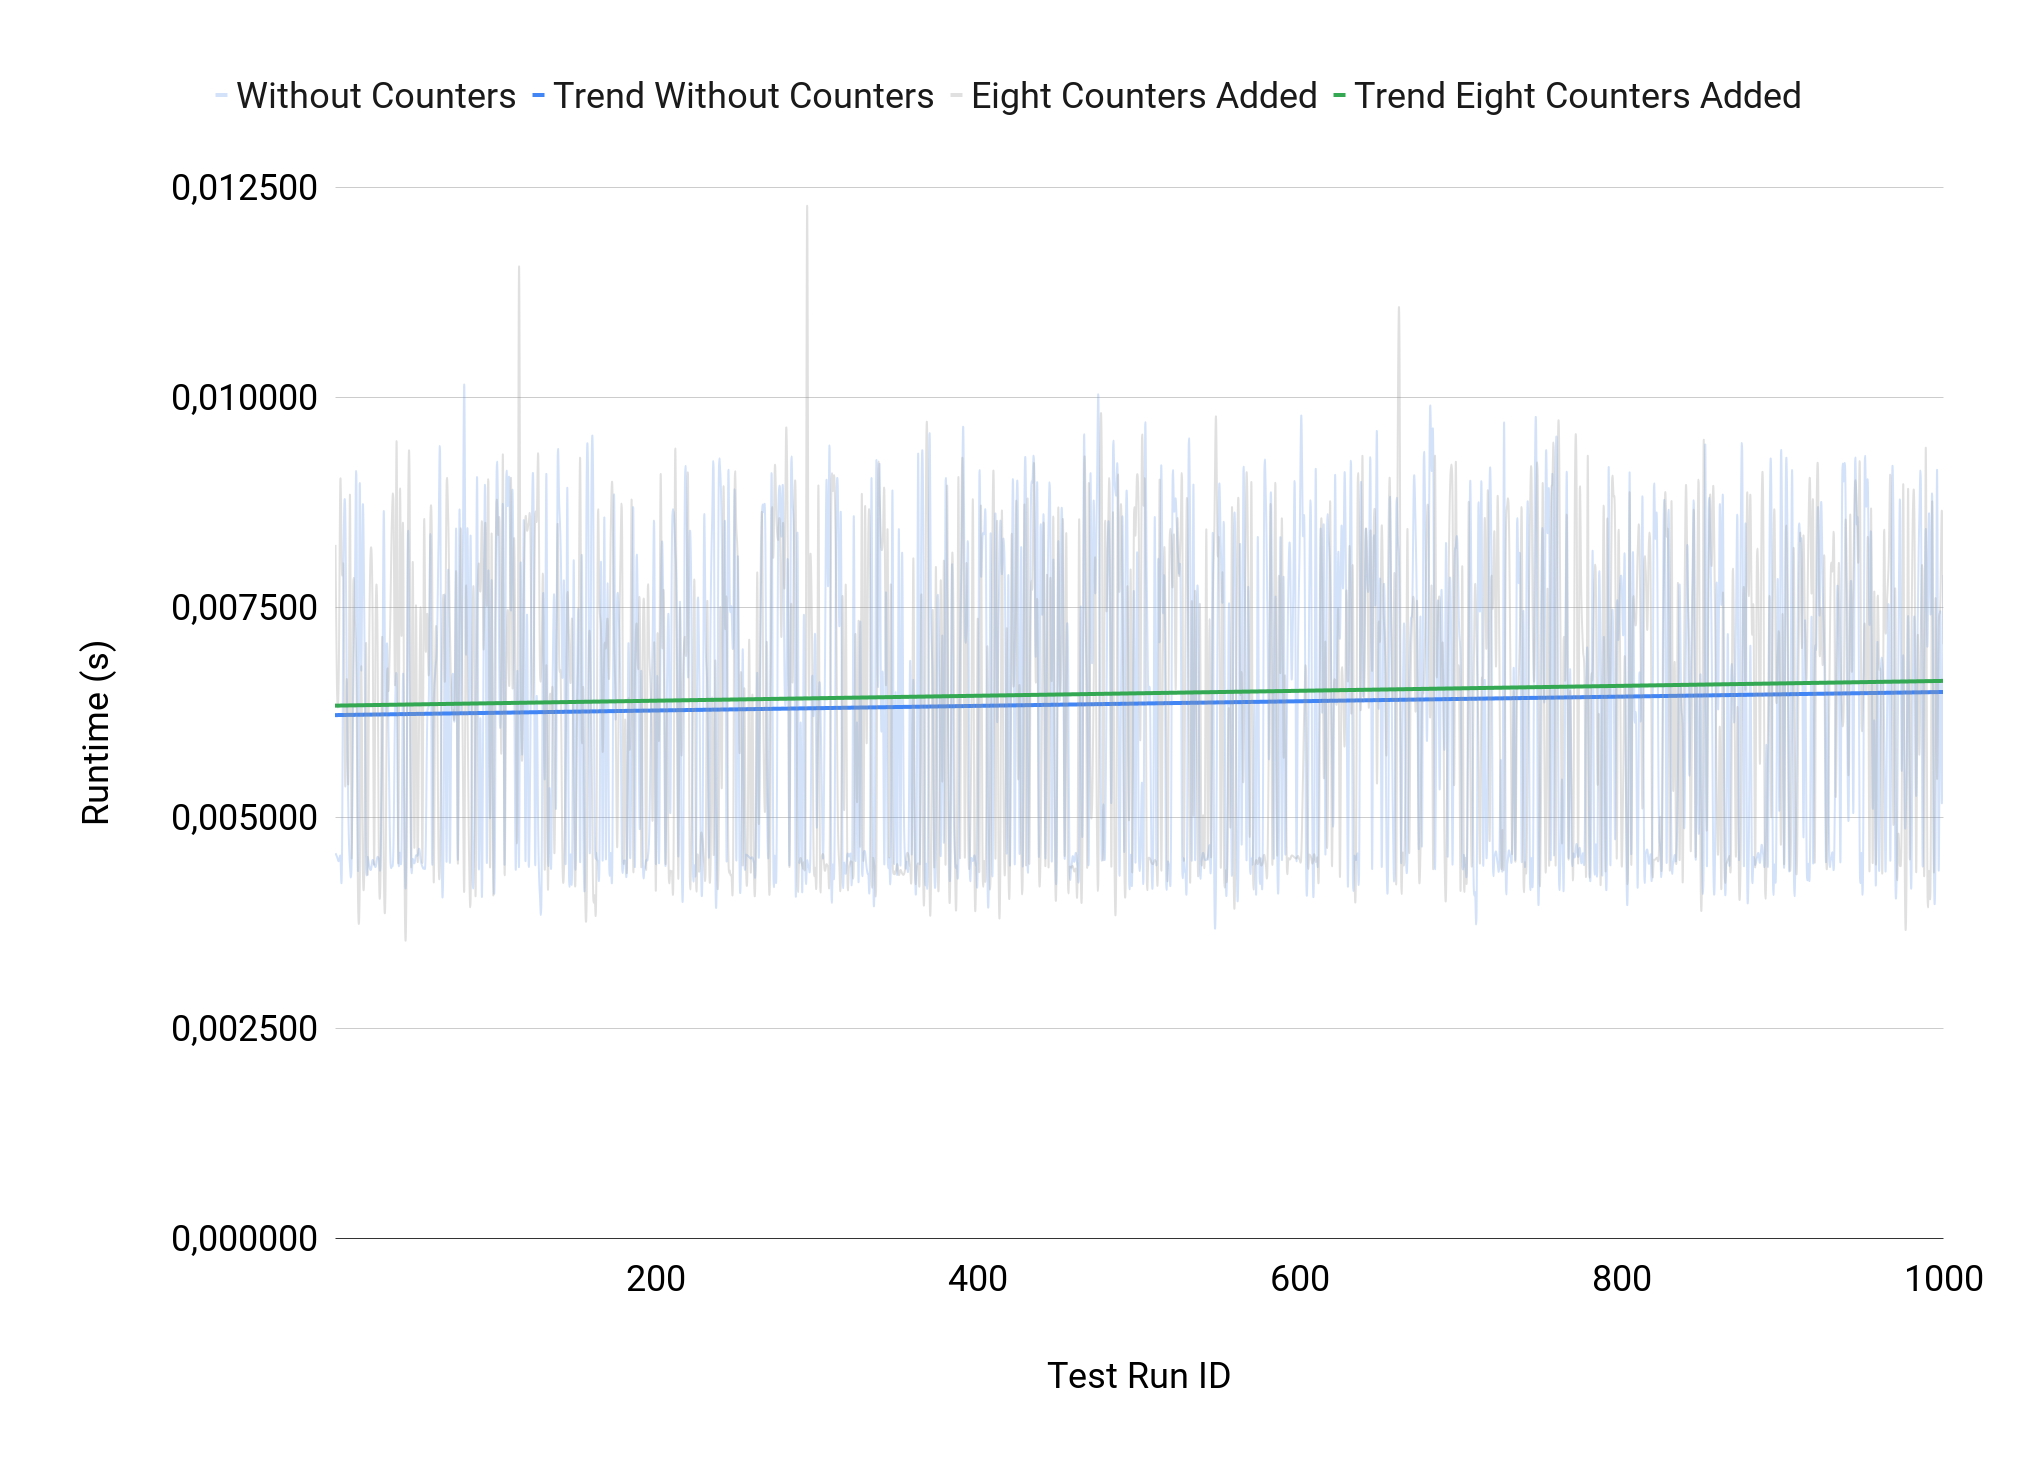
\includegraphics[width=1\textwidth]{graphics/e_forloop_comparison.png}
  \label{fig:e:forloop_comparison}
\end{figure}

\subsection{Varying Loop Runtimes}
First, the runtime of the \VARYINGLOOP~\ref{lst:e:perf_forloops} application will be examined, focusing on the times measured with the \CHRONO library, since \emph{gnu-time} can only achieve an accuracy of \SI{0.01}{\second}. For this reason, only the inserted performance counters can be examined in this analysis and the \lstinline{print()} function can be disregarded for the time being. The objective is to identify the difference in runtimes between the two program variants and to consider the time added per inserted performance counter.

The runtimes of each run performed on the AMD Ryzen test environment can be seen in Figure~\ref{fig:e:forloop_comparison}. The average of the durations of all runs without added performance counters is  \SI{16300}{\micro\second}, whereas the runtime after adding the performance counters is around \SI{16480}{\micro\second}, which in result is a deviation of \SI{180}{\micro\second}. In this example, a total of four \MEASUREPAIRS were recorded, whereby one measures the total running time and the other three the individual \lstinline{for}-loops. Thus it can be calculated that each \MEASUREPAIR consumed about \SI{45}{\micro\second} in this test environment. 

Figure~\ref{fig:e:forloop_environments} shows the average durations per run on the three test environments, once with counter added and once without counter added. It can be seen that on average the programs with added counters consumed \SI{0.34}{\percent}--\SI{2.28}{\percent} more time. If the increased time is calculated down to a single added performance counter, this results in a time of \SI{20}{\micro\second} for each \MEASUREVALUE taken across all environments. 

It can be stated that especially with programs that have a short runtime and only a few counters have to be added by the \TOOL, only a marginal deviation can be recognized. 

\begin{figure}[t]
  \centering
  \caption[Runtime Deviation for the \VARYINGLOOP Application.]{Runtime Deviation for the Execution of the \VARYINGLOOP Application. The diagram shows the increase in runtime in percent when eight counters are added. The test was performed on a \IMAC and a \MACBOOK and a \AMD.} 
  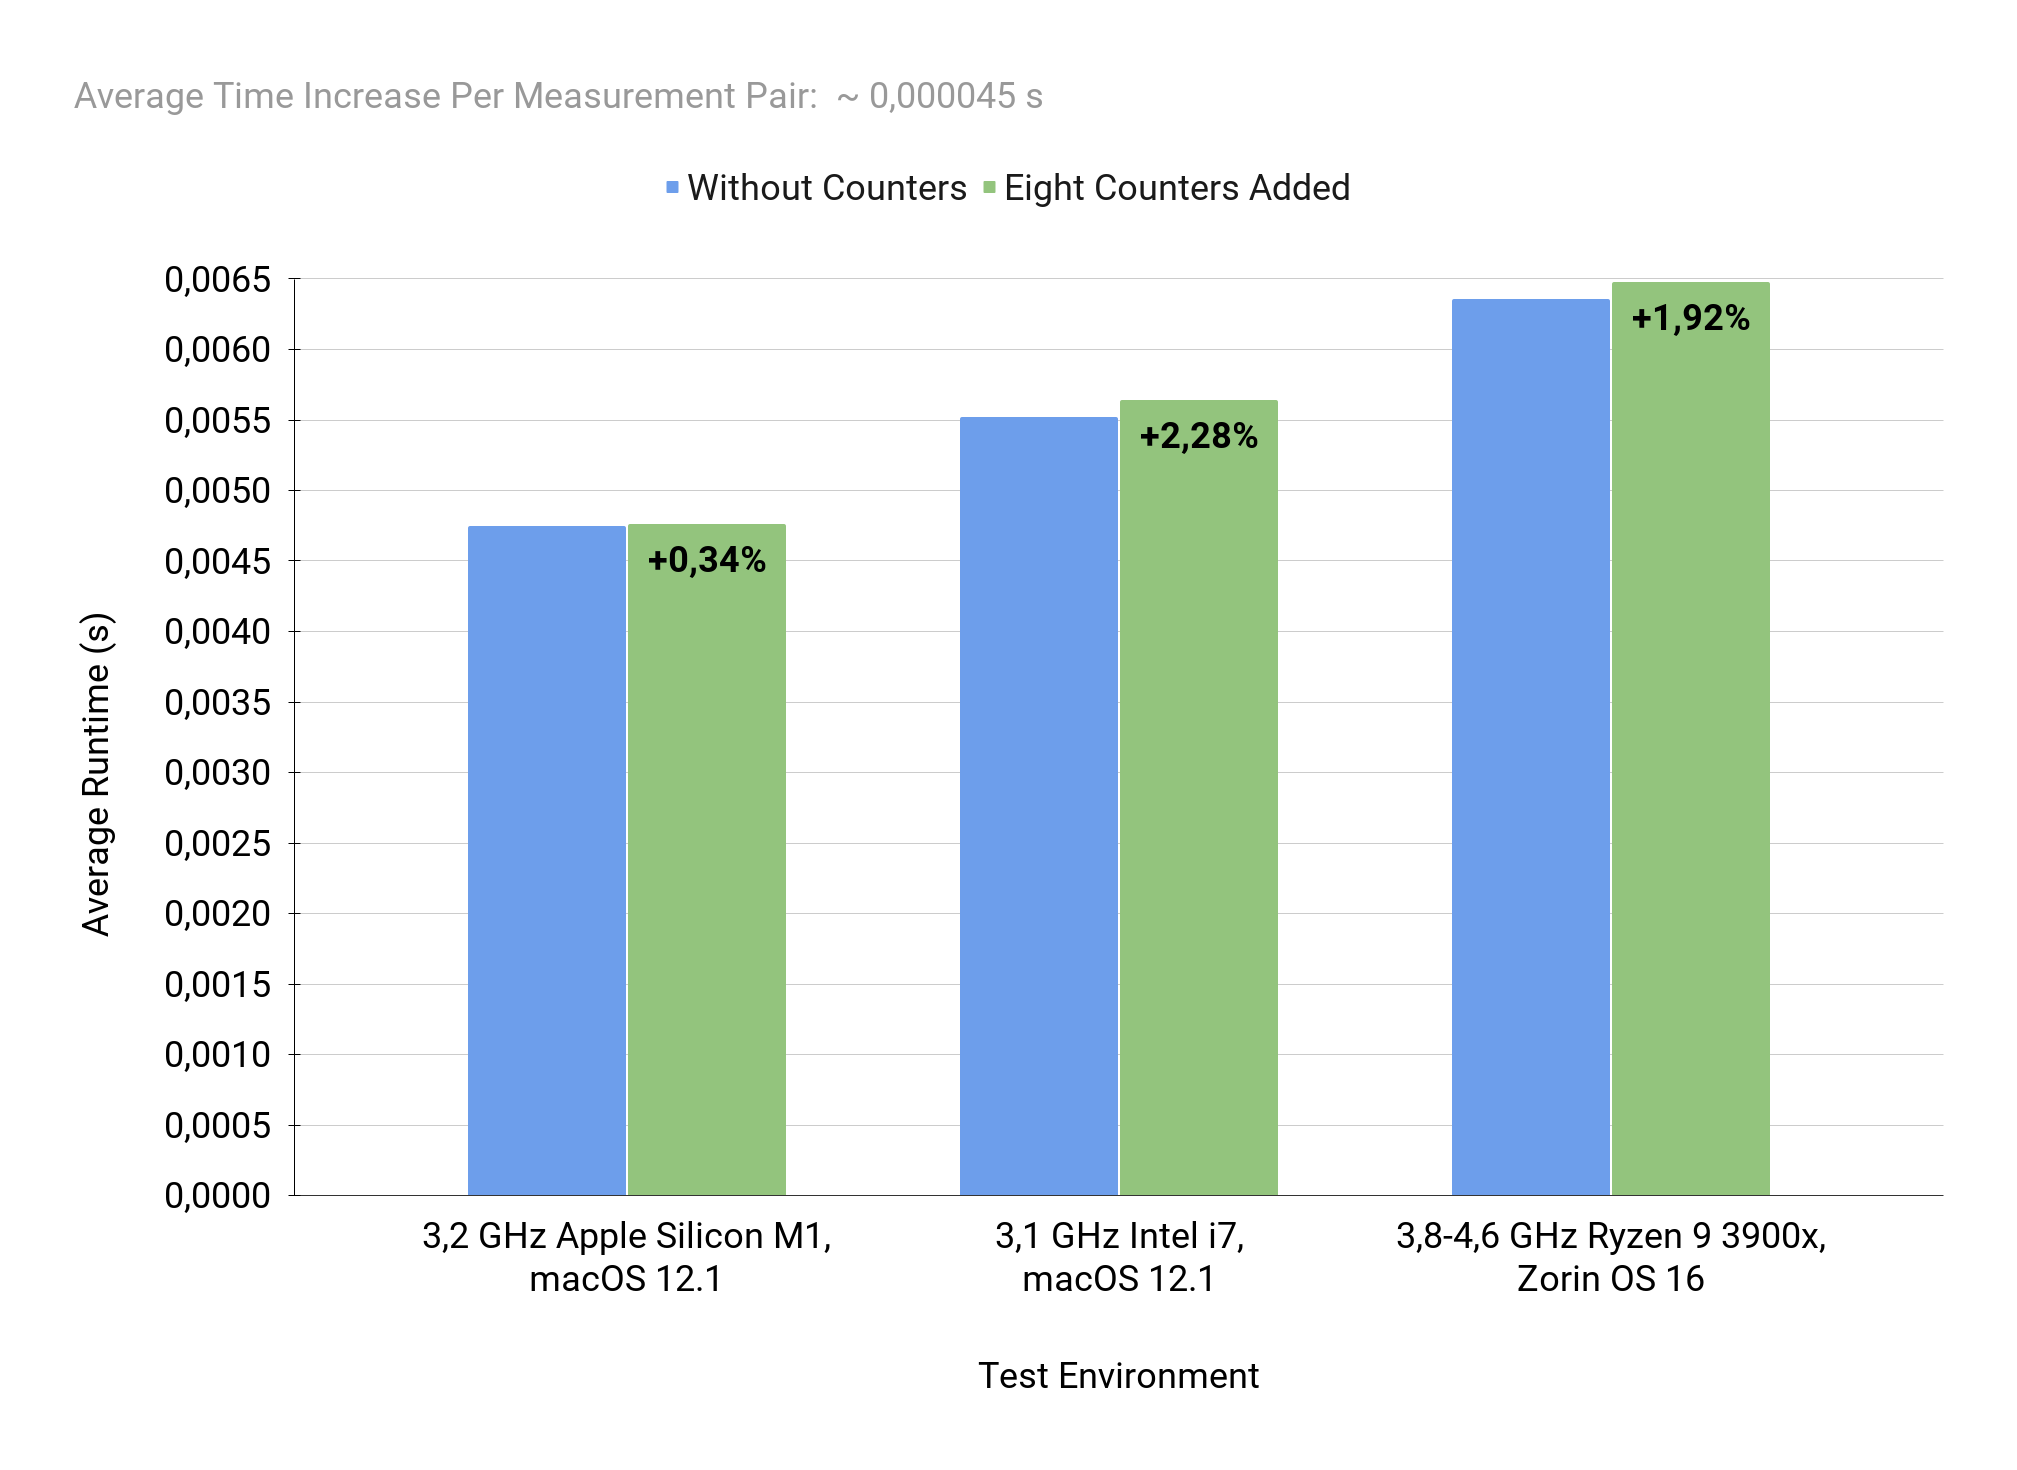
\includegraphics[width=1\textwidth]{graphics/e_forloop_environments.png}
  \label{fig:e:forloop_environments}
\end{figure}

\begin{figure}[t]
  \centering
  \caption[Runtime Comparison for the \FIBONACCI Application.]{Runtime Comparison for the \FIBONACCI Application. The runtime of the program without counters is compared to the version with eight counters added and the version with 4004 counters added. The Trend Lines Shown Represent the Average of the Runtimes Across All Test Environments. The test was performed on a \IMAC and a \MACBOOK and a \AMD.} 
  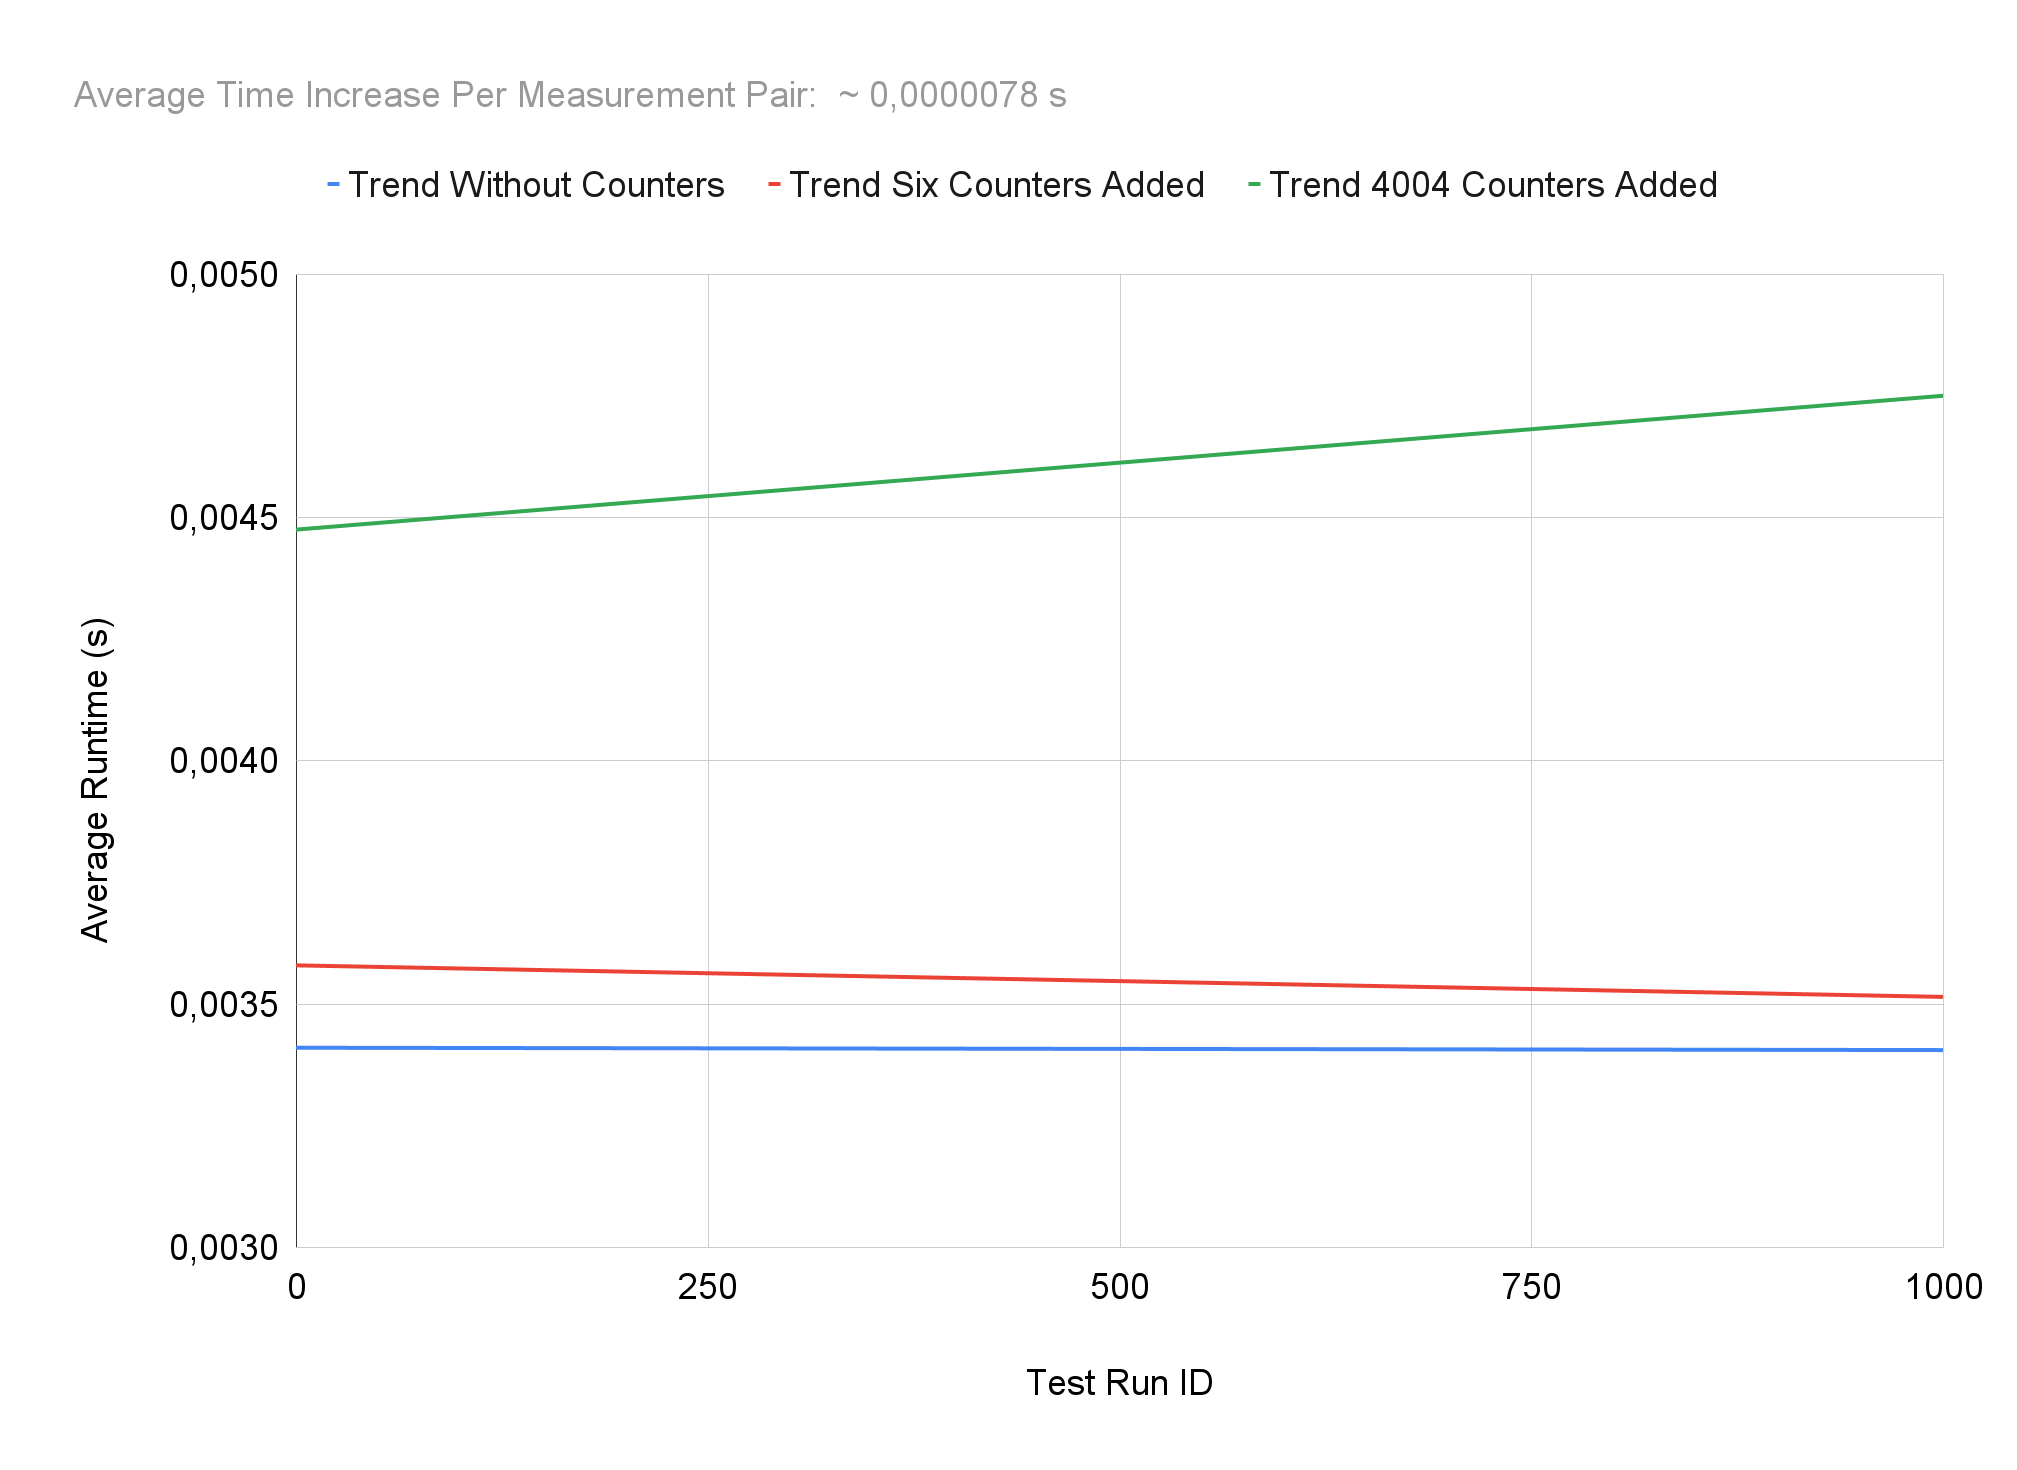
\includegraphics[width=1\textwidth]{graphics/e_fibonacci_comparison.png}
  \label{fig:e:fibonacci_comparison}
\end{figure}

\subsection{Fibonacci Sequence}
The \FIBONACCI~\ref{lst:e:perf_fibonacci} application that calculates the first thousand Fibonacci numbers will be looked at next. In contrast to the previous application, we showed in Section~\ref{sectionFibonacciCode} that two steps were needed to find the most resource-intensive part of the program. In the first step, the total running time and the duration of two single instructions were measured, which amounts to a total of three \MEASUREPAIRS or six \MEASUREVALUES recorded. In the second step, in addition to the total runtime, the runtime of the scope and two single instructions within a \lstinline{for}-loop were calculated. Since the \lstinline{for}-loop is executed exactly one thousand times and two instructions are measured within each, the total number of \MEASUREPAIRS is two thousand plus two pairs for the total and scope runtime, which amounts to 2002 \MEASUREPAIRS or 4004 \MEASUREVALUES. This example is intended to show that a distinction must be made between measurements that are performed only once and measurements that occur in a loop or a recursive function.

In Figure~\ref{fig:e:fibonacci_comparison}, the average runtimes of all environments for each run are given as trend lines. It can be seen that there is only a slight deviation between the variant without performance counter and the variant with six added \MEASUREVALUES. This difference amounts to an average of about \SI{4.11}{\percent} on all test environments. In the variant with 4004 \MEASUREVALUE recorded, on the other hand, a more significant increase in runtime of around \SI{39.22}{\percent} can be seen. It can be stated that in this example there seems to be no clear dependence between the number of \MEASUREVALUES recorded and the added runtime, since the deviations do not increase proportionally to each other. 

This behaviour can also be observed by looking at the average time increase per \MEASUREPAIR. The program version without added counters takes on average \SI{1136}{\micro\second}, the variant with six counters added around \SI{1182}{\micro\second} and the variant with 4004 counters added around \SI{1538}{\micro\second}. If we now calculate the average added per \MEASUREPAIR in this example, we get \SI{7,8}{\micro\second} per pair. However, it should be noted that a \MEASUREPAIR costs around \SI{15}{\micro\second} in the first step and only \SI{0.2}{\micro\second} in the second, although significantly more \MEASUREVALUES were recorded. This can be explained by the fact that the memory does not have to be reallocated with each loop pass, but only the current value has to be overwritten. 

Finally, the \TOTALCODEBLOCK can be considered. Although the costs of one \MEASUREPAIR is decreasing, the total time required to calculate the time of one code block is generally increasing. In the first step, the \TOTALCODEBLOCK cost around \SI{15}{\micro\second}, in the second step around \SI{100}{\micro\second}. This results from the fact that although the cost for a single \MEASUREVALUE is now lower, at the same time far more measurements are needed to calculate the time of one code block. Furthermore, it can also be stated that the execution time of the program is still very short and side effects caused by the hardware, the operating system or the time calculations of the runs can have a large impact on the final results. Consequently, the focus should shift to programs with a longer duration. Thus, we can take a closer look at the impact of the \MEASUREVALUES recorded on programs with a longer runtime.

\begin{figure}[t]
  \centering
  \caption[Runtime Comparison for the \PASSWORDGEN Application.]{Runtime Comparison for the \PASSWORDGEN Application. The Figure Shows The Average Runtime Over All Environments for Each Run. Program versions with a varying amount of added counters are compared to each other. The test was performed on a \IMAC and a \MACBOOK and a \AMD.} 
  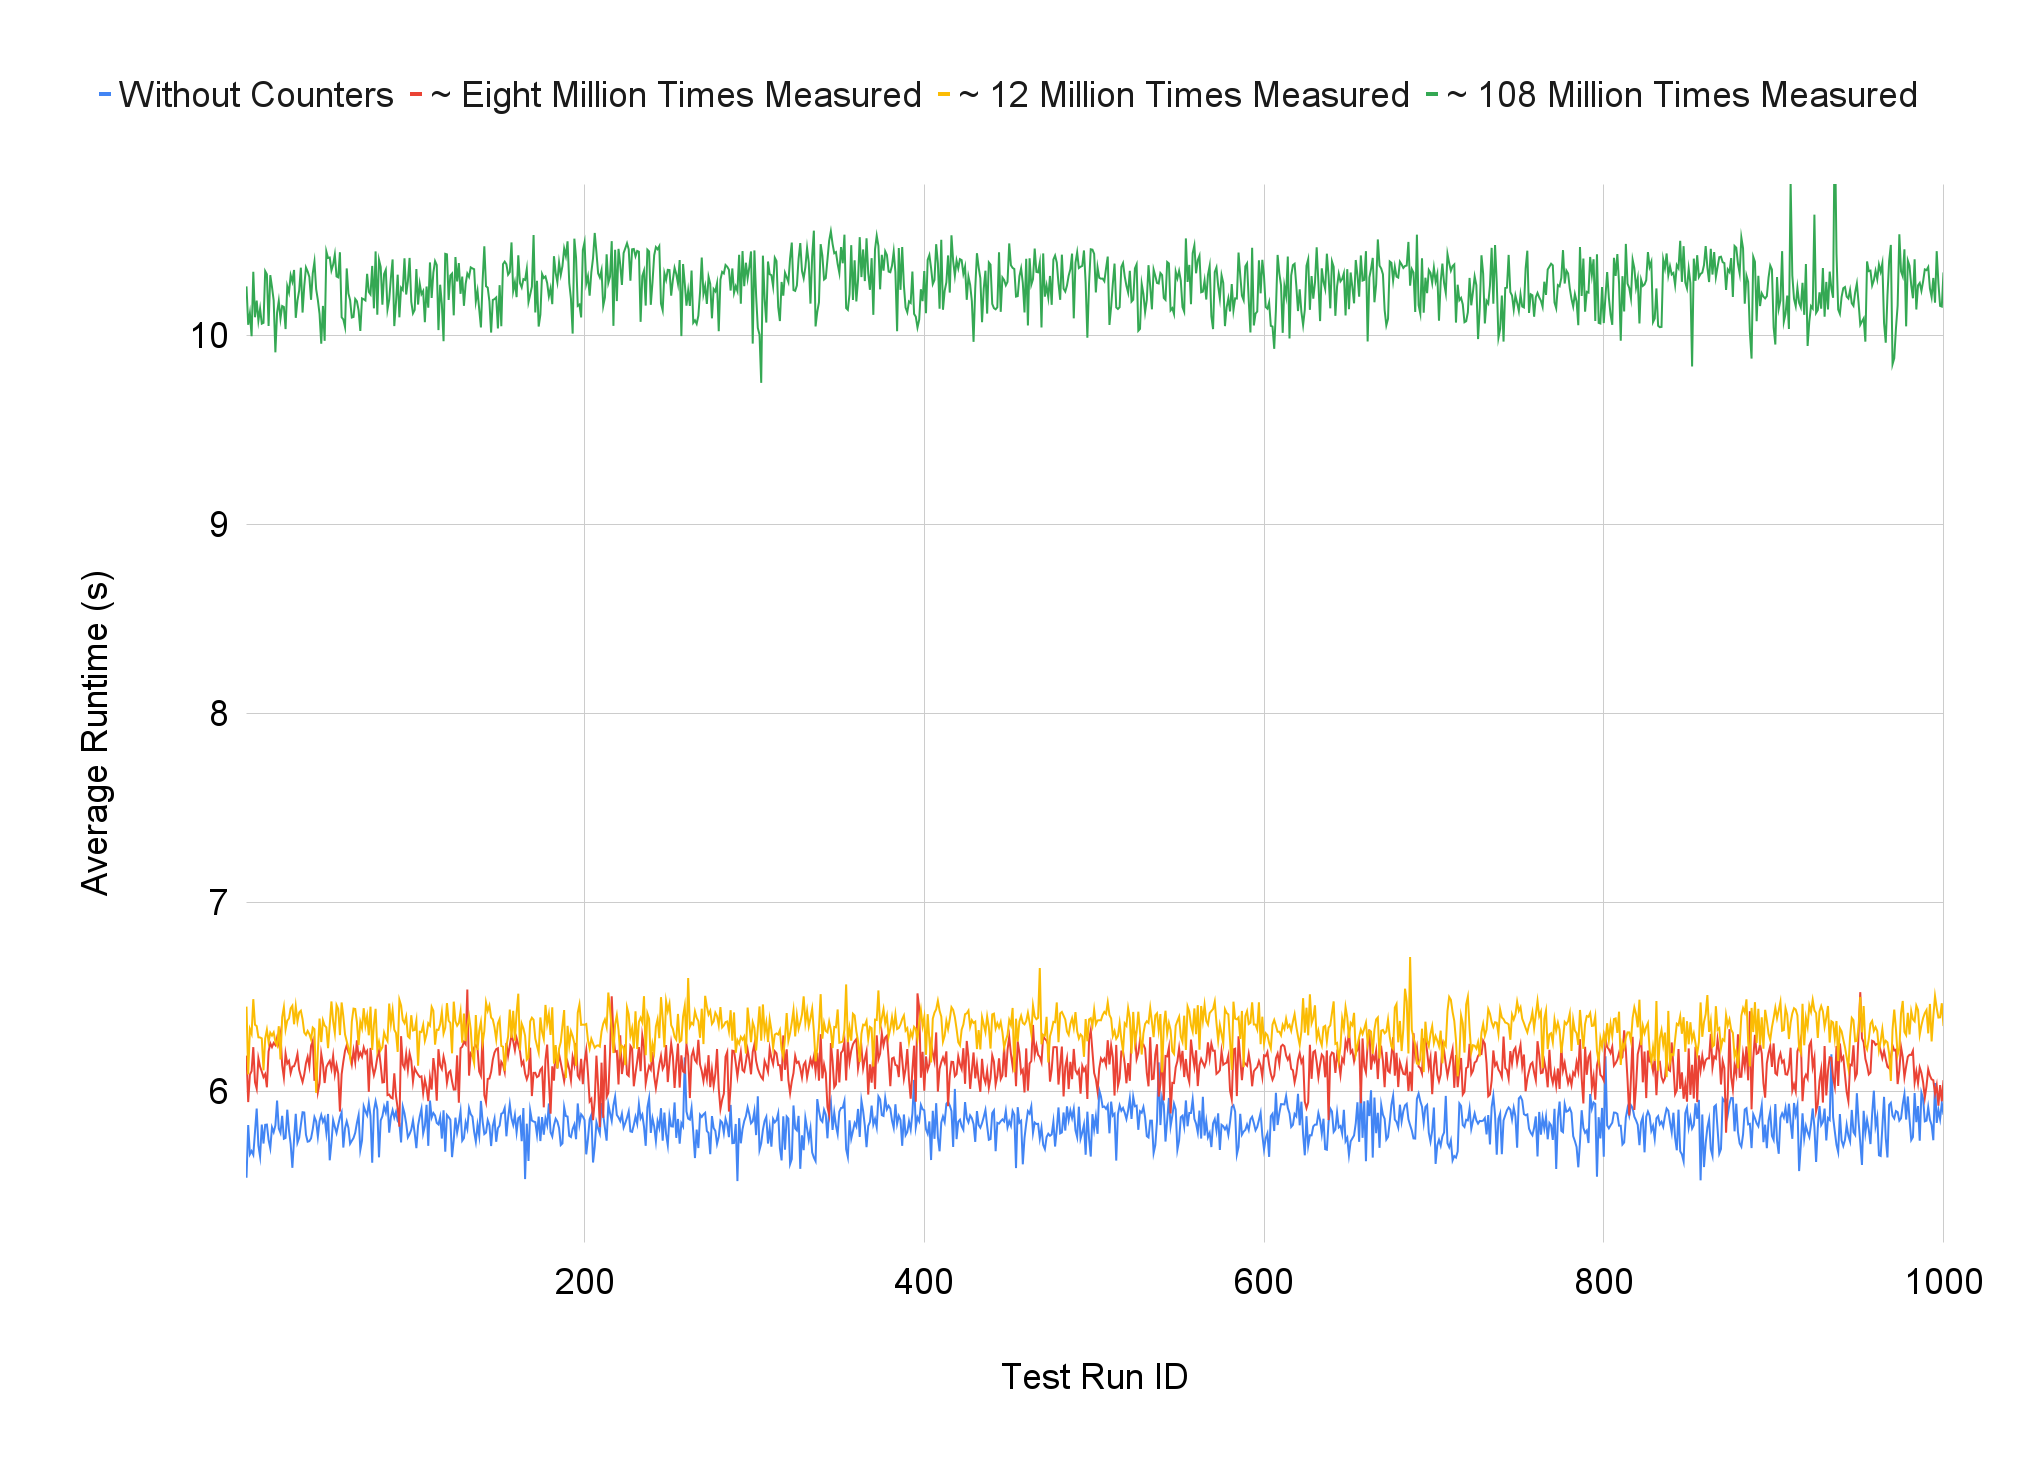
\includegraphics[width=1\textwidth]{graphics/e_password_comparison.png}
  \label{fig:e:password_comparison}
\end{figure}

\subsection{Password Generator}
The \PASSWORDGEN~\ref{lst:e:perf_passwords} application is to be examined next. We showed in Section~\ref{sectionPasswordCode} that a total of four steps were necessary in the profiling process to find the desired position in the code. In the first pass, eight \MEASUREVALUES were recorded for the time calculation of three code blocks, in the second eight million for the calculation of four code blocks, in the third fourteen million for calculating the time of two code blocks and in the last step 114 million for the calculation of three code blocks. The objective is to determine how the added performance counters affect programs with a longer runtime.

The average runtimes for each run across all test environments is shown in Figure~\ref{fig:e:password_comparison}. We have already discussed the deviations caused by a few added performance counters, so the first step is not considered for the following examples. The second step shows an increase in runtime of \SI{6.11}{\percent}, the third step an increase of \SI{10.68}{\percent} and the last step an increase of \SI{85.64}{\percent}. It can be noted that the increase scales approximately with the number of \MEASUREVALUES recorded. 

To view this effect from a different perspective, the average of the added time per \MEASUREPAIR can be calculated. The result is \SI{0.096}{\micro\second} per \MEASUREPAIR in step two, \SI{0.1}{\micro\second} in step three and \SI{0.092}{\micro\second} in step four, which amounts to an average of \SI{0.097}{\micro\second}. It can be seen that the runtime added per \MEASUREPAIR remains at approximately the same level or even decreases although more \MEASUREVALUES are taken in total. This can be explained by the fact that the allocation of memory for the individual data structure entries no longer has such a large influence on the result. In the previous example it could be seen that it has a big influence whether three or four \MEASUREPAIRS have to be allocated. However, in this application the deviation between the different numbers of \MEASUREPAIRS is negligible. 

In contrast, we want to look again at the time that must be spent to calculate the time of one code block. In the second step \SI{0.064}{\second} were spent, in the third step \SI{0.18}{\second} and in the last step \SI{1.05}{\second}. It can be seen that the \TOTALCODEBLOCK increases, since more calculations are needed to calculate the runtime of one code block. To investigate this further, the \PASSWORDGEN program will be modified so that a different number of passwords is added in each run. 

\subsection{Variable Password Size Generator}
For the \VARPASSWORDGEN Application the fourth step of the \PASSWORDGEN is to be adapted so that there is also a number of five data structure entries. This has the advantage that the difference caused by different numbers of data structure entries can be completely eliminated, since all runs have the same number of code blocks to be measured. Furthermore, the number of passwords should be randomly generated in the range from zero to two million so that any side effects caused by the hardware or the operating system can be distributed across all runs. Furthermore, the runs are now performed two thousand times to get a wider range of information. 

\begin{figure}[t]
  \centering
  \caption[Runtime Comparison for the \VARPASSWORDGEN Application.]{Runtime Comparison for the \VARPASSWORDGEN Application. The figure shows the increase of the runtime in relation to the generated passwords. The program version without added counters is compared to the version with counters and to the version with counters and \lstinline{print()} function. The test was performed on a \AMD. } 
  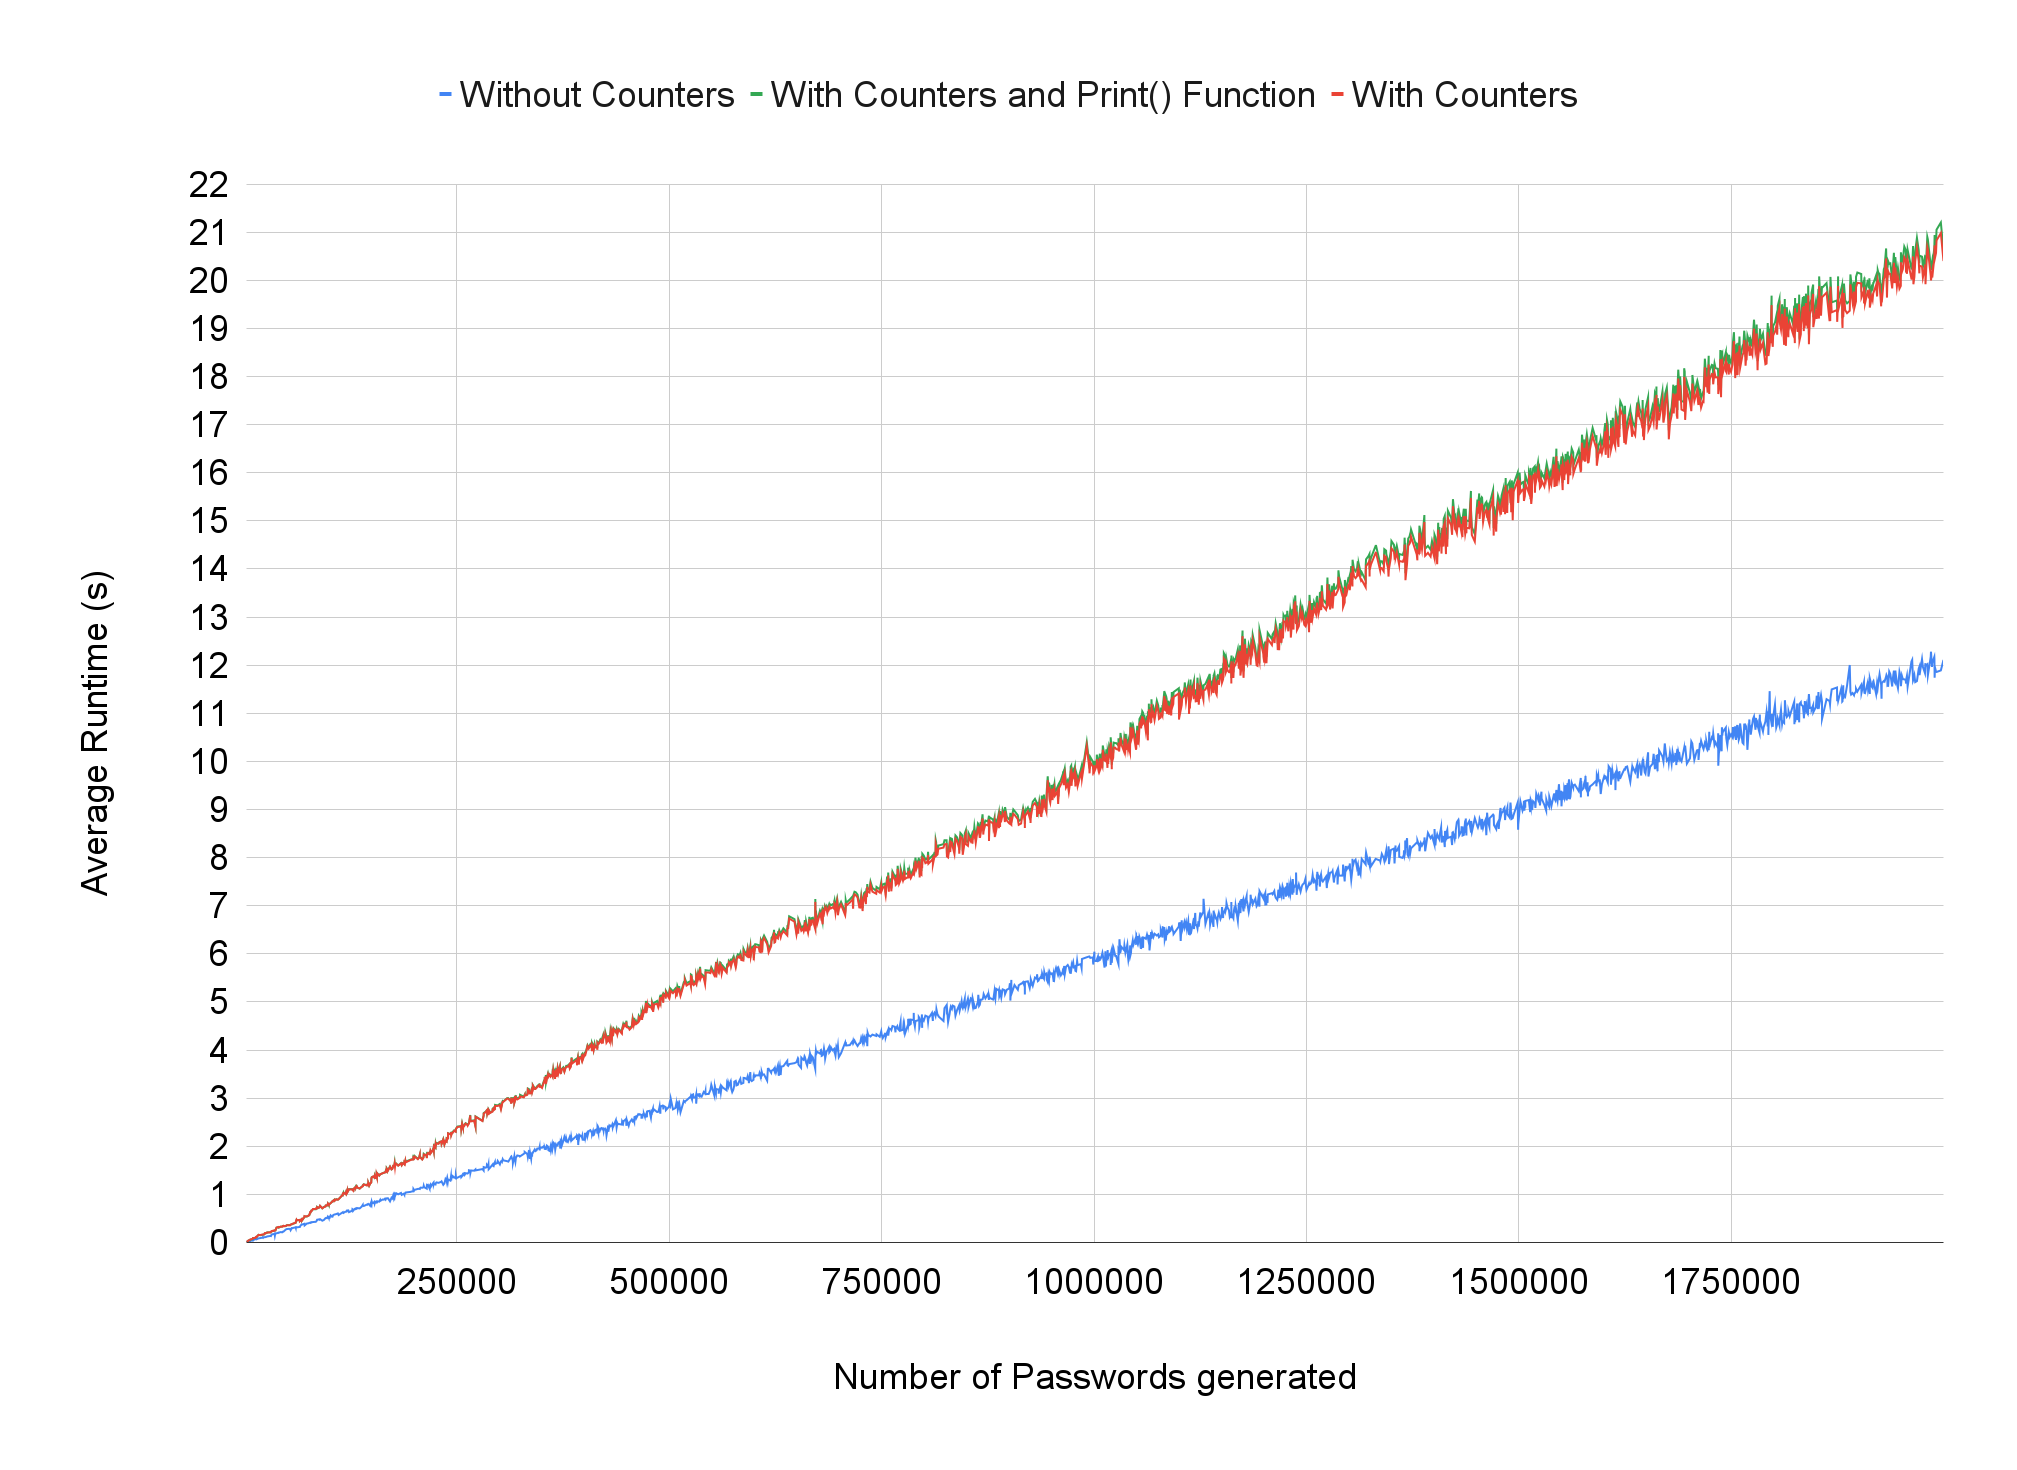
\includegraphics[width=1\textwidth]{graphics/e_variable_password_comparison.png}
  \label{fig:e:variable_password_comparison}
\end{figure}

Figure~\ref{fig:e:variable_password_comparison} shows the runtimes once with and once without added counters on the AMD Ryzen environment. In addition to the distinction between the program variants, a differentiation is now also made between the runtime of the counter itself and the runtime of the \lstinline{print()} function. On average, for five measured code blocks, the runtime of the \lstinline{print()} function is \SI{0.04}{\second} per run. Since in this example only a variable number \MEASUREVALUES are recorded, but the number of code blocks which runtime statistic is to be printed remains the same, the runtime of the \lstinline{print()} function does not change, but add a constant value to the total runtime. This is the case because the calculations of the runtimes of a loop are already made within the \lstinline{startEvent()} function, thus an enormous amount of resources can be saved since two separate timestamps do not have to be stored for each loop run. It can be noted that the runtime of the \lstinline{print()} function can only be increased by adding more code blocks to be measured, but adding single \MEASUREVALUES has no influence.

Furthermore, it should be calculated for all runs over all environments how much runtime is allocated to one \MEASUREVALUE. For this purpose, the total runtime can be divided by the number of performance counters used in this run. For the data of the program variant without inserted counters, the number of counters that would have been consumed can be calculated by scaling the number of passwords. An average value of \SI{0.06}{\micro\second} per \MEASUREVALUE can be calculated over the six thousand collected measurements. It can therefore be stated that a \MEASUREPAIR in this example costs around \SI{0.11}{\micro\second} of running time. Comparing this value with those of the previous examples, especially the second step in the \FIBONACCI program and step two to four in the \PASSWORDGEN application, it is noticeable that the deviation from the values calculated of these examples is very small. However, an average of \SI{1.3}{\second} was now spent calculating one code block. In the following we will compare the results of all programs in detail.

\begin{figure}[t]
    \centering
    \caption[Time Per \emph{Measurement Value} Comparison for Various Test Cases.]{Time Per \emph{Measurement Value} Comparison for Various Test Cases. The diagram shows the average time taken to record a \MEASUREVALUE. The \MEASUREVALUES calculated in the previous examples are compared to each other.}
    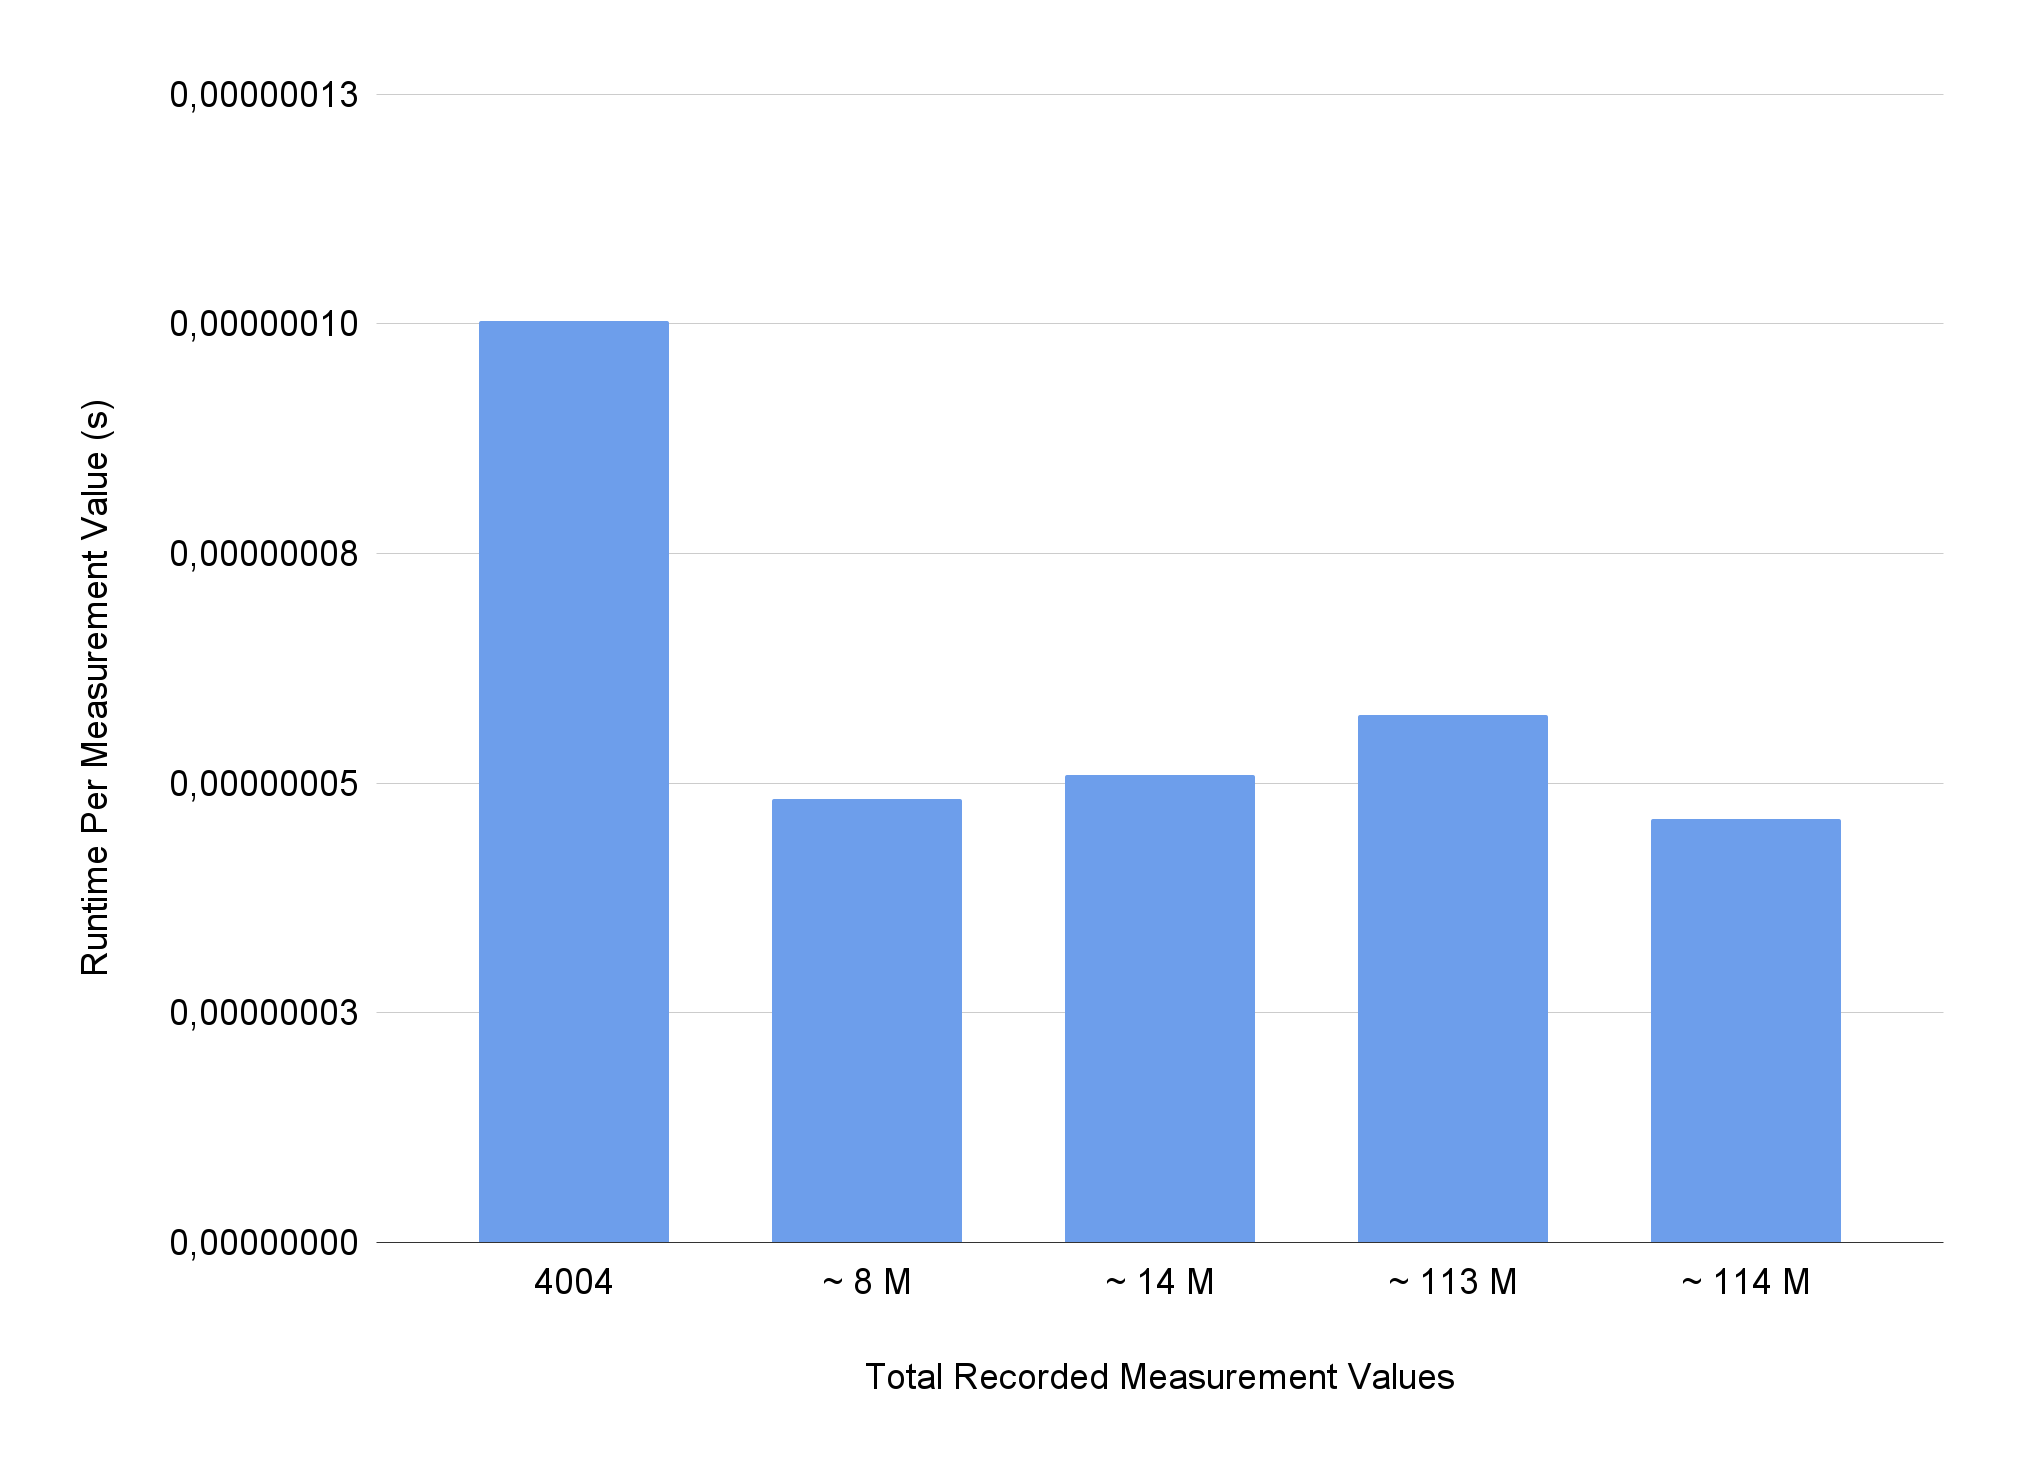
\includegraphics[width=\textwidth]{graphics/e_conclusion_per_counter.png}
    \label{fig:e:conclusion_per_counter}
\end{figure}
 
\subsection{Time Per Measurement And Total Overhead Per Code Block}
All values found for the runtime generated by one \MEASUREVALUE and the \TOTALCODEBLOCK of the various programs should be examined. Figure~\ref{fig:e:conclusion_per_counter} lists the additional times required per \MEASUREVALUE. It can be seen that this value stabilizes as more times are measured. The sum of the five considered values is \SI{0.06}{\micro\second}. Figure~\ref{fig:e:conclusion_per_array_entry} shows the \TOTALCODEBLOCK for all examples. These times increase as more \MEASUREVALUES are needed to calculate one code block. For the value calculated per \MEASUREVALUE, it can be said that it will not decrease further, but the \TOTALCODEBLOCK may greatly increase if more timestamps are measured and calculated.

\begin{figure}[t]
    \centering
    \caption[\emph{Total Overhead Per Code Block} Comparison for Various Test Cases.]{\emph{Total Overhead Per Code Block} Comparison for Various Test Cases. The diagram shows how much overhead was generated by the measurement of one code block. The \TOTALCODEBLOCK calculated in the previous examples are compared to each other.}
    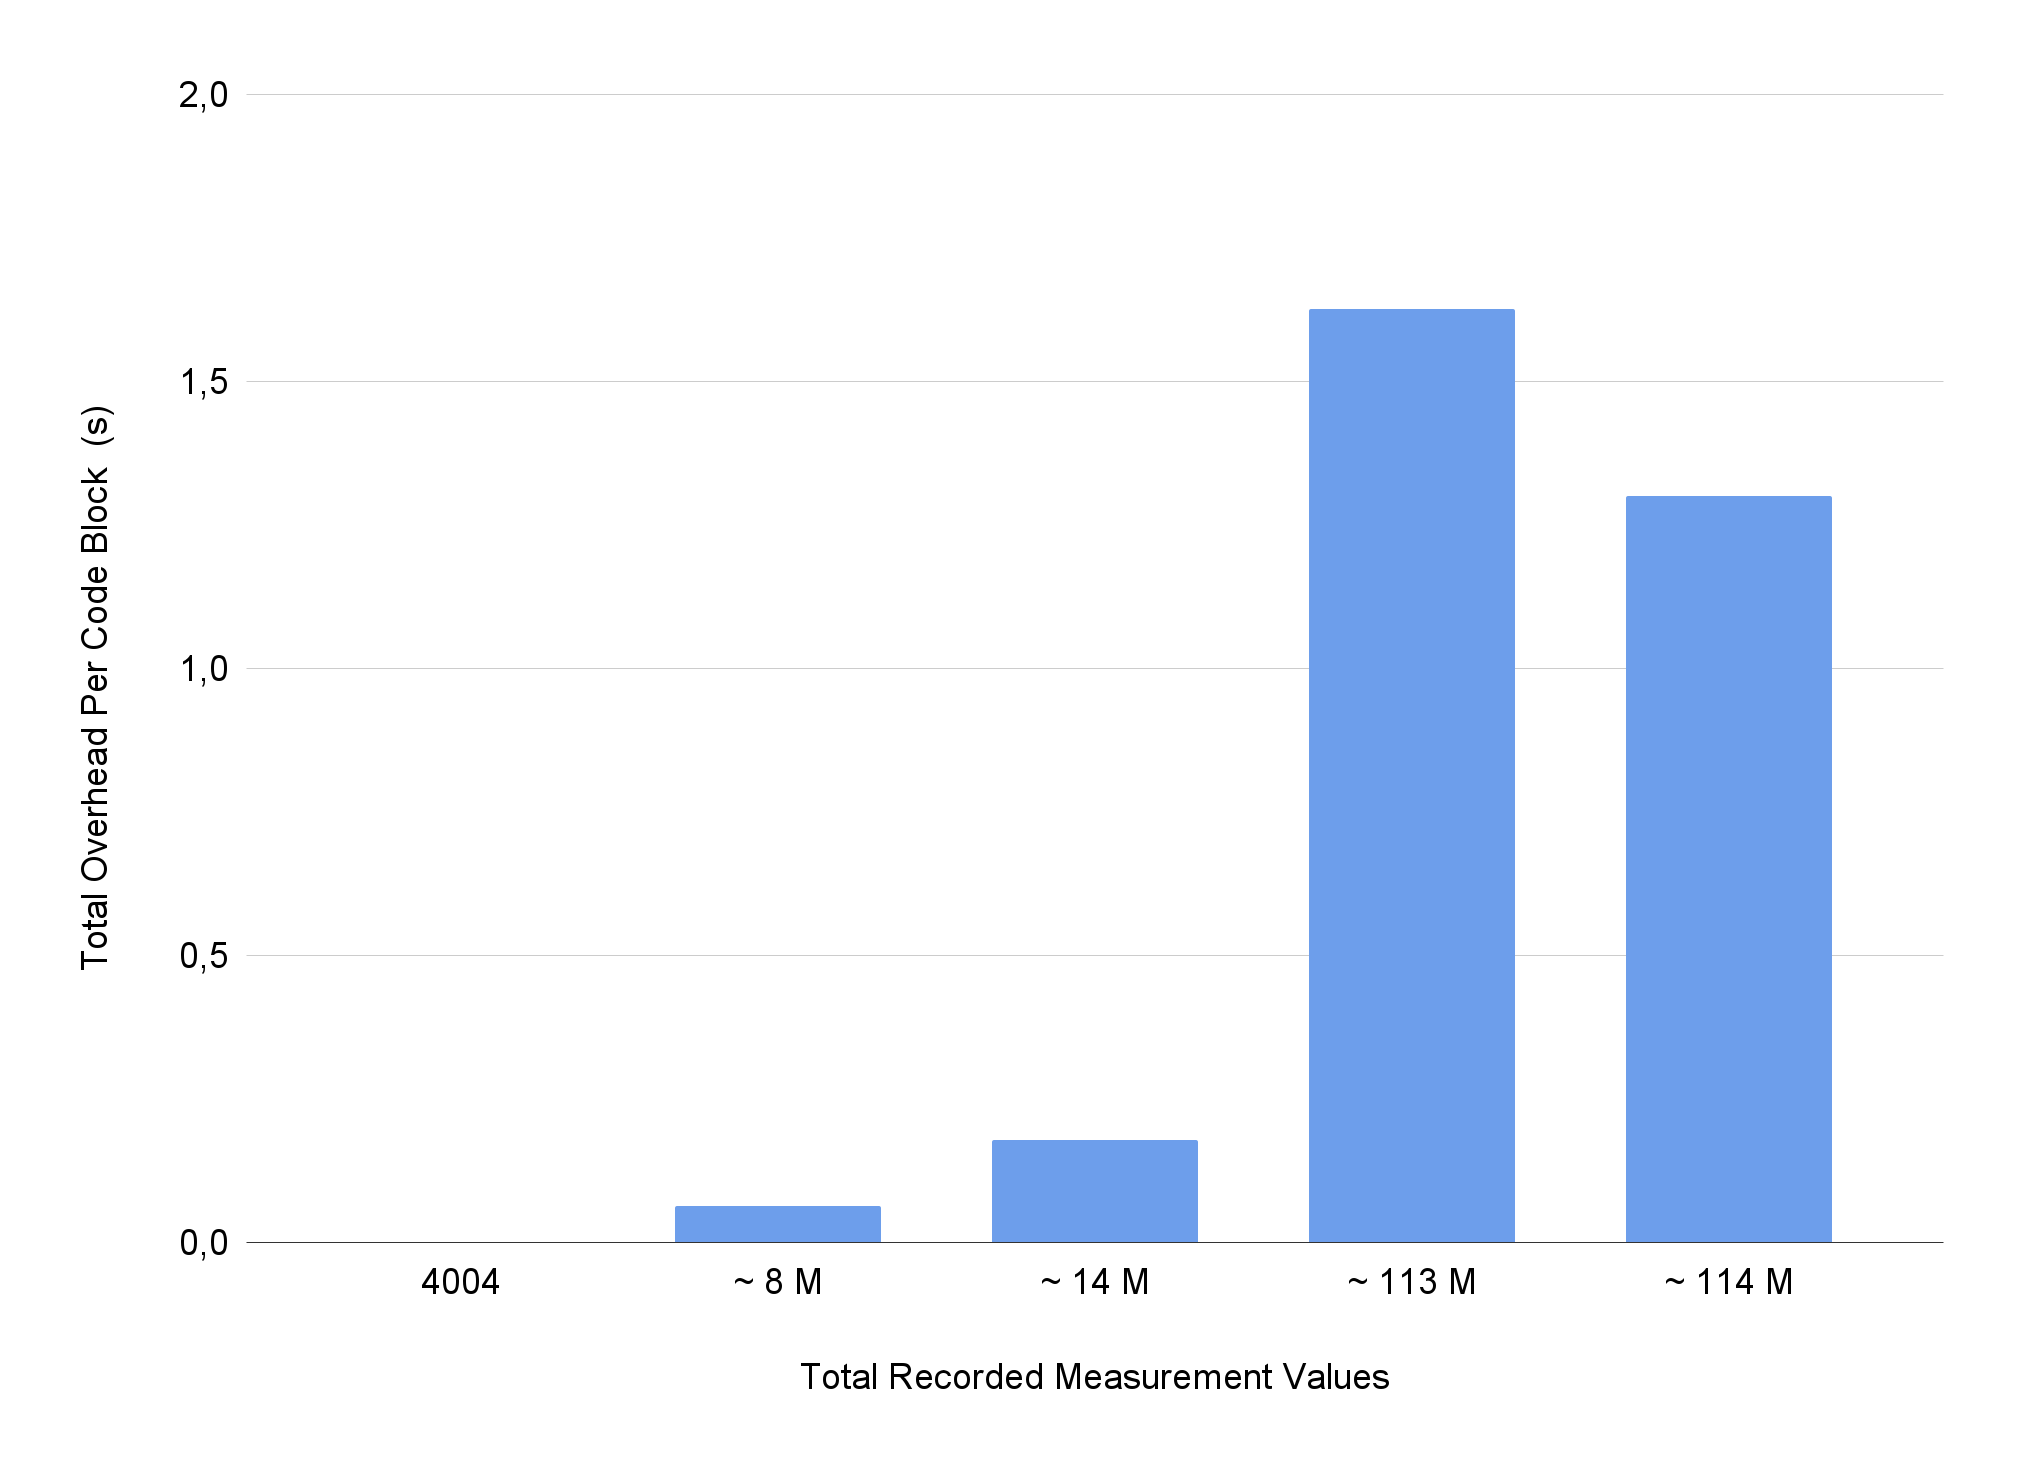
\includegraphics[width=\textwidth]{graphics/e_conclusion_per_array_entry.png}
    \label{fig:e:conclusion_per_array_entry}
\end{figure}

In conclusion, it can be stated that the performance of the tool depends on three parameters. The first one is the number of code blocks to be measured, which can be neglected especially if many measurements are carried out. The second parameter is the \TOTALCODEBLOCK. This value rise when more readings are needed to measure a single code block. The last parameter is the time taken by \MEASUREVALUE. It was found that this value stabilizes with a large number of measurements and drops below \SI{0.1}{\micro\second} after about a thousand measurements have been taken. It should also be noted that although the execution time of the program increases by inserting further measurements, the quality of the profiling process is not necessarily affected. On one hand, the \TOOL recognizes about half of the additional time consumed, even without further prediction models applied. On the other hand, the proportion of time consumed on one level enlarges evenly for all instructions, which means that statements can still be made about the most resource-intensive part of an application.  

\begin{figure}[t]
  \centering
  \caption[Prime Number Comparison for the \PRIME Application.]{Prime Number Comparison for the \PRIME Application. The diagram shows the ratio of calculated prime numbers to added performance counters. The runtime of all environments is compared to each other. The test was performed on a \IMAC and a \MACBOOK and a \AMD.} 
  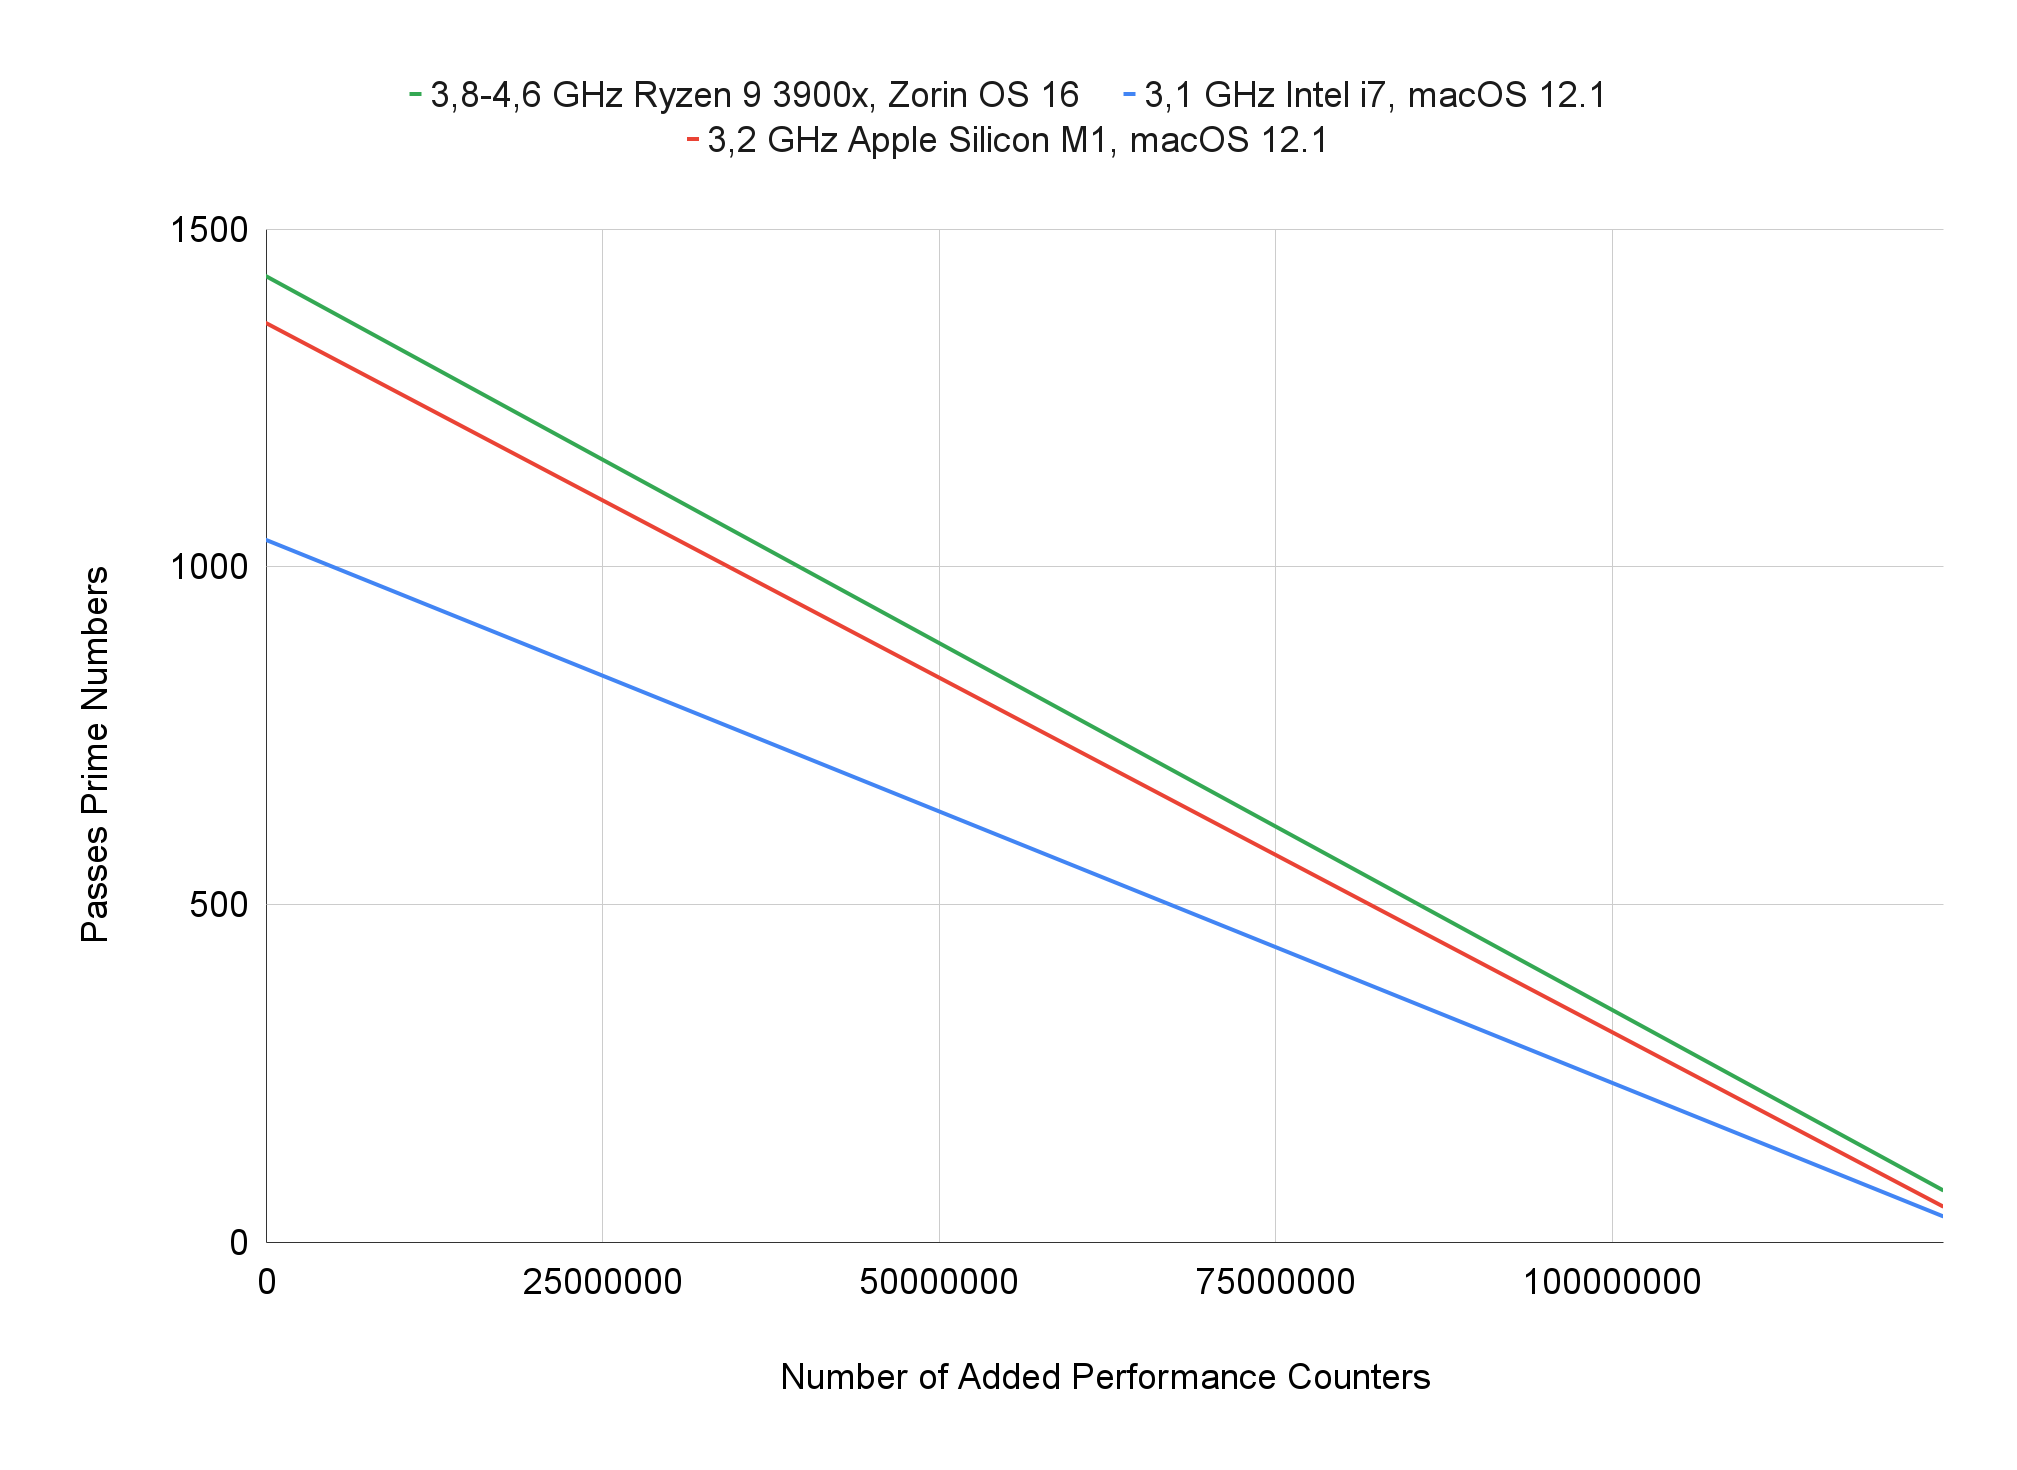
\includegraphics[width=1\textwidth]{graphics/e_prime_comparison.png}
  \label{fig:e:prime_comparison}
\end{figure}

\subsection{Prime Benchmark}
After all statements about the added time of the \TOOL have been made, the \PRIME~\cite{PrimeBenchmark} program will now be considered. In this example, no runtimes were measured, but rather calculated prime numbers. We showed in Section~\ref{sectionPrimeCode} that in order to reach the most resource-intensive part of the application, a total of six steps were required, whereby a different variable number of counters were inserted in each run, as this was dependent on the performance of the current run. In the first step, four \MEASUREVALUES were recorded, in the second, an average of 10241, in the third, a mean of 5105, in the fourth, approximately 1.2 million, in the fifth, an average of 0.8 million, and in the last step, an mean of 91 million. This test is particularly important to show that the \TOOL can also be used for any third-party application.

Figure~\ref{fig:e:prime_comparison} shows the results of the test on all environments, with a linear regression trend calculated across all steps. Since the first five readings are very close to each other, the values of these runs have to be looked at separately, but in general it can be seen that fewer prime numbers could be calculated by adding the counters. In the range from zero to ten thousand inserted counters, an average of 1280 prime numbers were calculated. In steps four and five, around 1260 primes were calculated in a range of 0.8--1.2 million inserted measurements. In the last step, with 91 million counters, only 56 prime numbers could be calculated. This can be explained by the fact that the time for the calculation of the prime numbers was not changed, but more counters were inserted, thus the time for the actual calculation approaches zero. 

For this specific application, it can be stated that the first five steps can be carried out without any problems, and only a slight performance drop can be detected. In the last step the calculation of the measured values takes more time than the calculations of the prime numbers themselves, whereby the performance drops enormously. Since a fixed runtime is used in this example, an infinite number of counters cannot be inserted, because at some point the profiling will take more time than the actual calculation of the prime numbers. However, we still succeeded in finding the most resource-intensive part of the program in Section~\ref{sectionPrimeCode}, since we were able to determine which part of the calculation takes the longest time, even when calculating only a few prime numbers. 